\documentclass[12pt,a4paper]{report}

% ========================================================
% ENGINE AND FONT SETTINGS
% Compile with XeLaTeX or LuaLaTeX
% ========================================================
\usepackage{iftex}
\ifPDFTeX
  \PackageError{main}{Please compile with XeLaTeX or LuaLaTeX}{Switch your compiler.}
\fi
\usepackage{fontspec}
\setmainfont{Times New Roman}
\setsansfont{Times New Roman}
\setmonofont{Courier New}

% ========================================================
% PACKAGES
% ========================================================
\usepackage[a4paper,margin=1in]{geometry}
\usepackage{setspace}
\usepackage{titlesec}
\usepackage[hidelinks]{hyperref}
\usepackage{graphicx}
\usepackage{array}
\usepackage{longtable}
\usepackage[table]{xcolor}
\usepackage{amsmath}
\usepackage{amssymb}
\usepackage{tocloft}
\usepackage{float}
\usepackage{caption}
\usepackage{booktabs}
\usepackage{enumitem}
\usepackage{ragged2e}
\usepackage{url}
\usepackage{microtype}
\usepackage{fancyhdr}
\usepackage{pdflscape}
\usepackage{multirow}


% ========================================================
% GLOBAL FORMATTING
% ========================================================
\onehalfspacing
\justifying
\setlength{\parindent}{0pt}
\setlength{\parskip}{6pt}
\renewcommand{\arraystretch}{1.25}
\setlength{\tabcolsep}{6pt}

\captionsetup{font=small,labelfont=bf,justification=centering}

\pagestyle{fancy}
\fancyhf{}
\fancyfoot[C]{\thepage}
\renewcommand{\headrulewidth}{0pt}

% ========================================================
% TOC FORMATTING
% ========================================================
\setcounter{tocdepth}{3}
\setcounter{secnumdepth}{3}
\renewcommand{\cftsecleader}{\cftdotfill{\cftdotsep}}
\renewcommand{\cftsubsecleader}{\cftdotfill{\cftdotsep}}
\renewcommand{\cftchapleader}{\cftdotfill{\cftdotsep}}
\setlength{\cftbeforechapskip}{8pt}
\setlength{\cftbeforesecskip}{4pt}
\setlength{\cftbeforesubsecskip}{2pt}
\renewcommand{\cfttoctitlefont}{\hfill\normalsize\bfseries}
\renewcommand{\cftaftertoctitle}{\hfill}
\renewcommand{\cftlottitlefont}{\hfill\normalsize\bfseries}
\renewcommand{\cftafterlottitle}{\hfill}
\renewcommand{\cftloftitlefont}{\hfill\normalsize\bfseries}
\renewcommand{\cftafterloftitle}{\hfill}
\titleformat{\chapter}[block]{\normalfont\normalsize\bfseries\centering}{\textbf{CHAPTER \thechapter:}}{0.5em}{\bfseries}
\titleformat{name=\chapter,numberless}[block]{\normalfont\normalsize\bfseries\centering}{}{0pt}{\bfseries}
\titlespacing*{\chapter}{0pt}{-10pt}{25pt}
\titleformat{\section}{\normalfont\large\bfseries}{\thesection}{1em}{}
\titleformat{\subsection}{\normalfont\normalsize\bfseries}{\thesubsection}{1em}{}
\titleformat{\subsubsection}{\normalfont\normalsize\itshape}{\thesubsubsection}{1em}{}
\setlist[itemize]{itemsep=4pt,topsep=4pt,leftmargin=1.2cm}
\setlist[enumerate]{itemsep=4pt,topsep=4pt,leftmargin=1.2cm}
\newcommand{\placeholderfigure}[2]{%
\begin{figure}[H]\centering\fbox{%
\begin{minipage}[c][6cm][c]{0.85\textwidth}\centering
\textbf{Figure Placeholder}\\[0.3cm]#2\\[0.3cm]
\textit{Replace with:} \texttt{\string\includegraphics[width=0.85\string\textwidth]\{name\}}
\end{minipage}}\caption{#1}\end{figure}}
\begin{document}
%% TITLE PAGE
\begin{titlepage}\thispagestyle{empty}\centering\vspace*{0.6cm}
{\Large\bfseries UNIVERSITY SOCCER LEAGUE MANAGEMENT\\ SYSTEM}\\[0.7cm]
{\large CASE STUDY: Mountains of the Moon University}\\[1.6cm]
%{\LARGE\bfseries PROJECT RESEARCH  REPORT}\\[1.2cm]
{\large\bfseries BY}\\[1cm]
\begin{tabular}{p{0.45\textwidth}p{0.45\textwidth}}
\centering\textbf{SANTO RAYERN} & \centering\textbf{MBAMBU ROSETTE}\tabularnewline
\centering 2023/U/MMU/BCS/01673 & \centering 2023/U/MMU/BIT/01795\tabularnewline
\centering Tel: 0750288271/0788674463 & \centering Tel: 0770408930\tabularnewline
\centering santorayern@gmail.com & \centering rossetmbambu9@mail.com\tabularnewline
\end{tabular}\\[1.2cm]
{\large\bfseries Supervisor: Samuel Ocen}\\
{\large Email: samuel.ocen@mmu.ac.ug}\\[1.4cm]
{\large A FINAL YEAR PROJECT REPORT SUBMITTED TO THE FACULTY OF SCIENCE, TECHNOLOGY AND INNOVATION,
IN PARTIAL FULFILLMENT OF THE REQUIREMENTS FOR THE\\ AWARD OF A BACHELOR'S DEGREE AT
\\MOUNTAINS OF THE MOON \\UNIVERSITY.}\\[1.5cm]
{\large\bfseries JUNE 2026}
\end{titlepage}
%% FRONT MATTER
\pagenumbering{roman}
\newpage\chapter*{DECLARATION}\addcontentsline{toc}{chapter}{Declaration}
We, \textbf{Santo Rayern} and \textbf{Mbambu Rosette}, declare that this project report titled
\textbf{``University Soccer League Management System : A Solution
for Soccer Operations at Mountains of the Moon University''} is our original work and has not been
submitted to any university or institution of higher learning for the award of any academic qualification.
\vspace{1.4cm}

\textbf{Student Name:} Santo Rayern\hfill\textbf{Reg. No.:} 2023/U/MMU/BCS/01673

\textbf{Signature:} \rule{7cm}{0.4pt}\hfill\textbf{Date:} \rule{4cm}{0.4pt}
\vspace{1.2cm}

\textbf{Student Name:} Mbambu Rosette\hfill\textbf{Reg. No.:} 2023/U/MMU/BIT/01795

\textbf{Signature:} \rule{7cm}{0.4pt}\hfill\textbf{Date:} \rule{4cm}{0.4pt}

\newpage\chapter*{APPROVAL}\addcontentsline{toc}{chapter}{Approval}
This project report titled \textbf{``University Soccer League Management System :
A Solution for Soccer Operations at Mountains of the Moon University''}
has been submitted for examination with my approval as the university supervisor.
\vspace{1.5cm}

\textbf{Supervisor Name:} Samuel Ocen

\textbf{Signature:} \rule{7cm}{0.4pt}\hfill\textbf{Date:} \rule{4cm}{0.4pt}
\vspace{1.4cm}

\textbf{Department:} Department of Computer Science

\textbf{Faculty:} Faculty of Science, Technology and Innovation

\textbf{Institution:} Mountains of the Moon University

\newpage\chapter*{DEDICATION}\addcontentsline{toc}{chapter}{Dedication}
This project is dedicated to our families, whose encouragement, sacrifice, prayers, and moral support
sustained us throughout our academic journey. We also dedicate this work to the students, sports
coordinators, coaches, referees, players, and spectators at Mountains of the Moon University, whose
participation and commitment to university sports inspired the development of UniLeague.

\newpage\chapter*{ACKNOWLEDGEMENT}\addcontentsline{toc}{chapter}{Acknowledgement}
We express our sincere gratitude to our supervisor, \textbf{Samuel Ocen}, for his guidance, patience,
constructive feedback, and support throughout this project.

We also thank the Faculty of Science, Technology and Innovation at Mountains of the Moon University
for providing an enabling academic environment. Special appreciation goes to the MMU sports community,
including sports coordinators, coaches, referees, players, and spectators, for sharing their experiences
during data collection and system evaluation.

Finally, we are grateful to our families and friends for their encouragement and continued motivation.

\newpage\tableofcontents
\newpage\listoftables\addcontentsline{toc}{chapter}{List of Tables}
\newpage\listoffigures\addcontentsline{toc}{chapter}{List of Figures}

\newpage\chapter*{LIST OF ABBREVIATIONS}\addcontentsline{toc}{chapter}{List of Abbreviations}
\begin{longtable}{p{3cm}p{11cm}}
API   & Application Programming Interface\\
AUUS  & Association of Uganda University Sports\\
BaaS  & Backend-as-a-Service\\
CRUD  & Create, Read, Update, Delete\\
DSR   & Design Science Research\\
EAUG  & Eastern Africa University Games\\
ERD   & Entity Relationship Diagram\\
FASU  & Federation of Africa University Sports\\
FEAUS & Federation of East African University Sports\\
FISU  & International University Sports Federation\\
HTTP  & HyperText Transfer Protocol\\
ICT   & Information and Communications Technology\\
JSON  & JavaScript Object Notation\\
JWT   & JSON Web Token\\
MMU   & Mountains of the Moon University\\
MVC   & Model-View-Controller\\
PWA   & Progressive Web Application\\
REST  & Representational State Transfer\\
RLS   & Row-Level Security\\
SQL   & Structured Query Language\\
SUS   & System Usability Scale\\
UAT   & User Acceptance Testing\\
UI    & User Interface\\
UX    & User Experience\\
WebSocket & Real-Time Communication Protocol\\
\end{longtable}

\newpage\chapter*{ABSTRACT}\addcontentsline{toc}{chapter}{Abstract}
University soccer league management at Mountains of the Moon University (MMU) in Fort Portal,
Western Uganda, was hindered by manual and fragmented administrative processes involving faculty-based
teams, registered players, match officials, and league coordinators. Existing operations relied on
informal WhatsApp communication, paper-based fixture records, spreadsheet player registers, and verbal
result reporting. These practices caused scheduling conflicts, delayed result reporting, poor performance
tracking, limited spectator engagement, and significant administrative burden on volunteer coordinators.

This study designed, developed, and evaluated a cross-platform University Soccer League Management
System --- \textbf{UniLeague} --- to improve soccer league operations at MMU. The study adopted a
Design Science Research approach supported by Agile software development. Requirements were gathered
using semi-structured interviews, observation, document review, questionnaires, and usability testing
involving sports coordinators, coaches, referees, players, and spectators.

UniLeague was implemented using Flutter for cross-platform user interfaces, Node.js and Express for
backend services, Supabase with PostgreSQL for centralised data storage, Prisma for object-relational
mapping, Provider for state management, Dio for HTTP communication, SQLite through \texttt{sqflite}
for offline local storage, and Socket.IO for real-time match updates. Security was strengthened using
Supabase authentication, row-level security, JWT-based authorisation, Helmet, CORS configuration,
and Zod validation.

Findings indicate that UniLeague reduces manual workload, centralises league data, improves fixture
and result management, supports evidence-based performance tracking, and enhances stakeholder
communication. The system offers a practical, cost-effective, and context-appropriate digital solution
adaptable by other resource-constrained universities in Uganda and East Africa.

\vspace{0.4cm}
\noindent\textbf{Keywords:} University sports management, soccer league management, cross-platform
application, fixture scheduling, real-time coordination, Flutter, Supabase, Design Science Research.

\newpage\pagenumbering{arabic}

%% ========================================================
%% CHAPTER ONE
%% ========================================================
\chapter{INTRODUCTION}
\section{Introduction}
This chapter presents the background and context of the university soccer league management system which is also called "UniLeague". It discusses global, continental,
regional, national, and institutional perspectives of university sports management, states the
problem that motivated the study, presents the objectives and research questions, defines the
scope, and explains the significance of the project.

\section{Background of the Study}
University sports serve as platforms for student development, institutional branding, physical
fitness, talent identification, and community engagement. Soccer, being one of the most popular
sports among university students, requires effective coordination of teams, players, fixtures,
match officials, results, standings, and performance records.

Globally, university sports operate under structured governance frameworks that increasingly
depend on digital systems for scheduling, coordination, and performance management. The
International University Sports Federation (FISU), founded in 1949, serves as the global
governing body for university sport and promotes sport events, education, student well-being,
and sustainability as key strategic pillars \cite{fisu2023,fisu_strategy2031}. Digital management tools have
become important in improving data accuracy, administrative efficiency, and decision-making
in sports programs \cite{fonti2023}.

In Africa, university sports are coordinated at continental level by the Federation of Africa
University Sports (FASU). Despite this governance structure, many African universities still
manage sports activities manually due to limited financial resources, lack of appropriate digital
systems, and inadequate technical infrastructure \cite{fasu2024}. Manual systems often lead to
fragmented records, delayed communication, poor result tracking, and weak performance analysis.

At regional level, the Federation of East African University Sports (FEAUS) coordinates
university sports activities across East African countries. However, many institutions in the
region still rely on paper records, spreadsheets, WhatsApp groups, and verbal communication to
manage sports competitions \cite{feaus2024,feaus_objectives}. These approaches are difficult to audit, prone to
errors, and unsuitable for systematic performance tracking.

In Uganda, university sports are coordinated through bodies such as the Association of Uganda
University Sports (AUUS) \cite{ncs_act2023,auus2020}. Although smartphone use and internet access continue
to increase, many university sports programs still lack dedicated digital platforms for league
management.

Mountains of the Moon University in Fort Portal, Western Uganda, faces similar challenges.
The university soccer league is managed through manual and fragmented processes involving paper
fixture lists, spreadsheets, informal WhatsApp communication, and verbal result submission.
These processes make it difficult to generate conflict-free fixtures, maintain accurate player
records, track match results, calculate standings promptly, and provide spectators with timely
information. This situation motivated the development of UniLeague.

\section{Problem Statement}
Soccer league management at Mountains of the Moon University was critically hindered by manual,
fragmented, and unauditable administrative processes. Operations involving faculty-based teams,
registered players, match officials, coaches, and league coordinators relied on paper records,
spreadsheets, WhatsApp messages, and verbal reporting.

This approach created several operational challenges. Fixture generation was done manually,
resulting in scheduling conflicts and frequent changes. Player registration data was stored in
disconnected spreadsheets, leading to duplicate and incomplete records. Match results were
reported late or verbally, making standings inaccurate or outdated. Substitution and match event
communication lacked audit trails, causing disputes among stakeholders. Spectators also lacked
reliable access to fixtures, results, and league standings \cite{sarlak2024}.

Therefore, there was a need to develop an integrated cross-platform soccer league management
system that could automate fixture scheduling, centralise team and player records, support
real-time match coordination, track performance statistics, provide accurate league standings,
and improve spectator engagement in a cost-effective and contextually appropriate manner.

\section{Objectives of the Study}
\subsection{Main Objective}
To develop a soccer league management system,that
streamlines league administration, enables real-time match coordination, provides structured
performance tracking, and enhances spectator engagement at Mountains of the Moon University.

\subsection{Specific Objectives}
\begin{enumerate}
  \item To analyse the current soccer league management processes at Mountains of the Moon University.
  \item To design the soccer league management system .
  \item To implement the designed soccer league management system.
  \item To test and evaluate the new soccer league management system.
\end{enumerate}

\section{Research Questions}
\begin{enumerate}
  \item What limitations existed in the current soccer league management processes at MMU?
  \item What system architecture, database design, and user interface approach were suitable for
        an integrated soccer league management system at MMU?
  \item How effectively did the developed system implement automated fixture generation, match
        coordination, performance tracking, and spectator engagement features?
  \item To what extent did the developed system reduce administrative burden, improve data
        accuracy, enhance communication, and achieve user acceptance among stakeholders?
\end{enumerate}

\section{Scope of the Study}

\subsection{Physical Scope}
The study was physically conducted at Mountains of the Moon University (MMU) located in
Fort Portal City, Western Uganda. All system development, prototyping, testing, and pilot
evaluation activities were carried out within the MMU campus environment, using the
university's soccer league operations as the primary case study.

\subsection{Content Scope}
The study focused on soccer league management functions including team registration, player
registration, fixture scheduling, match result entry, match event recording, substitution
management, league standings, player and team statistics, notifications, and spectator
access. The system did not cover financial management, ticketing, medical records, betting,
live video streaming, or multi-sport tournament management.

\subsection{Technical Scope}
UniLeague was developed as a cross-platform system using Flutter for mobile and web
interfaces, Node.js and Express for backend services, Supabase with PostgreSQL for database
services and authentication, Prisma for database access, SQLite through
\texttt{sqflite} for offline local storage, and Socket.IO for real-time communication.
The system supports role-based access for administrators, coaches, referees, players,
and spectators. The system did not include payment processing, biometric verification,
or live video streaming.

\subsection{Time Scope}
The project was conducted over an eighteen-week period from March 2026 to July 2026,
covering requirements analysis, system design, backend and frontend development,
integration, testing, deployment, pilot evaluation, and report writing.

\section{Significance of the Study}
\subsection{To Sports Administrators}
UniLeague helps sports administrators reduce manual workload by centralising registration,
fixtures, results, standings, and reports, improving data access and supporting faster
decision-making.

\subsection{To Coaches and Team Captains}
The system enables coaches and captains to manage team information, view fixtures, monitor
player records, and track team performance throughout the league.

\subsection{To Referees}
UniLeague provides structured tools for recording match events such as goals, cards,
substitutions, and final scores, reducing errors and improving the reliability of match records.

\subsection{To Players}
Players benefit from access to fixtures, results, standings, and individual performance
statistics, which can improve motivation and participation.

\subsection{To Spectators}
Spectators can access updated league information including fixtures, results, tables, and match
updates through a public portal, improving engagement and interest in university soccer.

\subsection{To Researchers and Developers}
The study contributes to knowledge on context-aware sports management systems in
resource-constrained university environments and can guide future research and software
development projects in digital sports administration \cite{vec2024}.

\section{Organisation of the Report}
This report is organised into six chapters. Chapter One presents the introduction, background,
problem statement, objectives, research questions, scope, significance, and organisation.
Chapter Two reviews related literature on theoretical frameworks, scheduling algorithms,
digital systems, cross-platform technologies, and existing system gaps. Chapter Three explains
the research methodology. Chapter Four presents system analysis and design. Chapter Five
presents system implementation, testing, and evaluation. Chapter Six provides results,
conclusions, recommendations, limitations, and areas for future work.

%% ========================================================
%% CHAPTER TWO
%% ========================================================
\chapter{LITERATURE REVIEW}
\section{Introduction}
This chapter reviews literature related to university sports management, soccer league
administration, theoretical frameworks, scheduling algorithms, digital sports management
systems, cross-platform development, backend technologies, database systems, real-time
communication, offline-first design, security, testing, and existing systems. The chapter
also identifies gaps that justify the development of UniLeague.

\section{Theoretical Frameworks}
\subsection{Sports Information Systems Theory}
Sports information systems are digital platforms designed to collect, process, store, and
distribute sports-related information. They support administrative functions such as
registration, scheduling, communication, result tracking, and performance analysis \cite{sarlak2024}.
The development of UniLeague was guided by three main principles: automation of repetitive
administrative tasks, centralisation of fragmented data, and accessibility for non-technical users.

\subsection{Design Science Research Framework}
Design Science Research (DSR) provides a framework for creating and evaluating information
technology artefacts that solve real organisational problems \cite{hevner2004}. Since this
study produced a working software system, DSR was suitable because it emphasises problem
identification, artefact design, demonstration, evaluation, and communication of results.

\subsection{Agile Software Development}
Agile methodology supports iterative development, continuous feedback, and incremental delivery
of software \cite{pressman2019}. This approach was appropriate because stakeholder requirements
evolved as coordinators, coaches, and referees interacted with prototypes.

\subsection{User-Centered Design}
User-centered design focuses on developing systems based on the needs, abilities, and
limitations of actual users. Since MMU soccer operations involve stakeholders with varying
levels of digital literacy, user-centered design was important in creating simple,
task-oriented interfaces.

\section{Review of University Sports and League Management}

\subsection{University Sports Management}
University sports management involves planning, organizing, coordinating, monitoring, and
evaluating sports activities within a higher education institution \cite{sarlak2024}. It
includes athlete registration, team formation, scheduling, facility allocation, officiating,
communication, result management, disciplinary control, and performance monitoring.

\subsection{Soccer League Administration}
A soccer league requires structured management of teams, players, fixtures, referees, match
venues, scores, standings, disciplinary actions, and performance statistics. Fixture scheduling
is one of the most important tasks in league administration. Manual fixture generation can
become complex as the number of teams increases \cite{vanbulck2022}.

\section{Review of Scheduling Algorithms}
\subsection{Round-Robin Scheduling}
Round-robin scheduling is commonly used in sports leagues because each team plays against every
other team in a structured sequence. It is simple, predictable, and suitable for small to
medium-sized leagues \cite{ribeiro2010}. However, basic round-robin scheduling does not
automatically detect venue, time, or team availability conflicts.

\subsection{Constraint Satisfaction and Metaheuristics}
Constraint satisfaction approaches generate fixtures while checking conditions such as venue
availability, team schedules, and fairness rules \cite{davari2020}. Integer programming,
tabu search, and genetic algorithms have also been applied to sports scheduling problems
\cite{vanbulck2022,rasmussen2008}. For a university system operated by non-technical users,
a simplified round-robin algorithm with constraint checking was more practical.

\begin{table}[H]
\centering
\caption{Summary of Reviewed Scheduling Algorithm Studies}
\begin{tabular}{p{3.5cm}p{3cm}p{4cm}p{3cm}}
\toprule
\textbf{Author/Year} & \textbf{Focus} & \textbf{Strengths} & \textbf{Limitations}\\
\midrule
Van Bulck \& Goossens (2022) & Integer programming & Produces optimal schedules & Requires expert config\\
Davari \& Goossens (2020) & Constraint satisfaction & Handles complex constraints & Complex UI\\
Rasmussen \& Trick (2008) \cite{rasmussen2008} & Tabu search & High constraint satisfaction & Slow and technical\\
Ribeiro \& Urrutia (2010) & Round-robin & Fast and easy to understand & Needs conflict detection\\
\bottomrule
\end{tabular}
\end{table}

\section{Review of Related Technologies}

\subsection{Digital Transformation in Sports}
Digital transformation in sports refers to the use of ICT to improve sports operations,
communication, performance analysis, and fan engagement \cite{fonti2023}. At university level,
digital transformation can improve basic administration and participation. A digital sports
management system can reduce paperwork, improve data accuracy, and provide timely access to
information.

\subsection{Sports Management Information Systems}
A sports management information system is a software platform used to collect, process, store,
and distribute sports-related information \cite{sarlak2024}. The effectiveness of such a
system depends on usability, reliability, accessibility, data security, and alignment with
user needs. User-centered design is therefore important in sports systems.

\subsection{Cross-Platform Application Development}
Cross-platform development allows developers to build applications that run on multiple
platforms using a shared codebase. Flutter is a cross-platform framework by Google that
enables the development of mobile, web, and desktop applications from a single codebase
\cite{flutter2024}. In UniLeague, Flutter was selected to support both mobile and web
access while reducing development time.

\subsection{Backend Technologies for Sports Systems}
Node.js is commonly used for scalable network applications because it supports event-driven,
non-blocking I/O programming. Express provides a lightweight framework for building RESTful
APIs \cite{nodejs2024}. Prisma was used as an object-relational mapping tool to simplify
database queries and improve maintainability.

\subsection{Database Management and Supabase}
PostgreSQL is a powerful open-source relational database system suitable for structured data
management \cite{postgresql2024}. Supabase provides a hosted PostgreSQL database,
authentication services, APIs, and row-level security policies. In UniLeague, Supabase was
used to provide centralised storage, authentication support, and fine-grained access control.

\subsection{Offline-First Design}
Offline-first design allows an application to continue performing important functions even
when internet connectivity is poor or unavailable \cite{sarlak2024}. UniLeague uses SQLite
through \texttt{sqflite} for offline local storage and \texttt{connectivity\_plus} to monitor
connectivity status.

\subsection{Real-Time Communication}
Socket.IO supports real-time bidirectional communication between clients and servers
\cite{socketio2024}. In UniLeague, it was used to provide real-time match updates and
notifications, improving stakeholder engagement and reducing delays in information sharing.

\subsection{System Security}
UniLeague uses authentication, role-based authorisation, Supabase row-level security,
JWT-based access control, input validation, CORS configuration, and secure HTTP headers
through Helmet \cite{helmet2024}. Zod validation ensures that data submitted through
forms and APIs follows expected formats.

\subsection{Testing and Evaluation}
Software testing may include unit testing, widget testing, integration testing, usability
testing, and user acceptance testing \cite{pressman2019}. The System Usability Scale (SUS)
is a widely used instrument for measuring usability through standardised Likert-scale
questionnaires \cite{brooke1996}.

\section{Review of Existing Systems}
\subsection{Commercial Sports Management Platforms}
Commercial platforms such as TeamSnap, LeagueApps, and SportsEngine are often designed for
commercial leagues, require subscription fees, assume reliable internet access, and may be
too complex for volunteer-managed university leagues.

\begin{table}[H]
\centering
\caption{Comparative Analysis of Existing Commercial Platforms \cite{fortune2024}}
\begin{tabular}{p{3cm}p{4cm}p{6cm}}
\toprule
\textbf{Platform} & \textbf{Strengths} & \textbf{Limitations for MMU Context}\\
\midrule
TeamSnap & Mobile interface, team messaging & Costly; lacks strong fixture automation\\
LeagueApps & Administrative automation & Designed for fee-based commercial leagues\\
SportsEngine & Comprehensive sports tools & Expensive; requires technical setup\\
OpenTournament & Open-source & No real-time updates; no offline support\\
Tourney Master & Tournament scheduling & Limited to tournaments; no full league\\
\bottomrule
\end{tabular}
\end{table}

\subsection{Open-Source and Academic Prototypes}
Open-source systems reduce licensing costs but often lack mobile interfaces, real-time
communication, or offline capability. Academic prototypes demonstrate individual components
but do not integrate all required features into one practical platform for resource-constrained
universities.


\section{Literature as per Specific Objectives}

\subsection{Literature Related to Objective One: Analysing Current Processes}
Studies on manual university sports administration highlight challenges such as fragmented
records, delayed communication, fixture conflicts, and lack of reliable statistics
\cite{sarlak2024,pmc2023}. These findings informed the analysis of MMU's current soccer
league management processes and helped identify specific gaps that the system would address.

\subsection{Literature Related to Objective Two: System Design}
Literature on cross-platform development, offline-first design, relational databases, and
user-centred design informed the system architecture and interface design. Flutter was
selected for its ability to support Android, iOS, and web from a single codebase
\cite{vec2024,flutter2024}. Supabase PostgreSQL and Prisma were selected based on their
suitability for structured relational data with strong access control \cite{postgresql2024,supabase2024}.

\subsection{Literature Related to Objective Three: System Development}
Agile development, RESTful APIs, Socket.IO real-time communication, PostgreSQL, and SQLite
informed the implementation of the system \cite{xu2024,socketio2024}. These technologies
supported real-time communication, centralised storage, and offline access in resource-
constrained environments.

\subsection{Literature Related to Objective Four: Testing and Evaluation}
Usability testing, System Usability Scale, system testing, and user acceptance testing
informed the evaluation approach \cite{brooke1996,pressman2019}. Studies on digital
sports management evaluation showed that ease of use, usefulness, and stakeholder
satisfaction are key metrics for system acceptance \cite{sarlak2024,smith2023}.

\section{Identified Literature Gap}
Table~\ref{tab:litgap} summarises the analysis of existing literature and the specific gaps
that this research addressed.

\begin{longtable}{p{2.4cm}p{3.0cm}p{2.8cm}p{3.2cm}p{2.8cm}}
\caption{Literature Review Gap Analysis}
\label{tab:litgap}\\
\toprule
\textbf{Author \& Year} & \textbf{Focus of Study} & \textbf{Strengths} &
\textbf{Weaknesses / Gaps} & \textbf{Relevance to This Study}\\
\midrule
\endfirsthead
\multicolumn{5}{l}{\small\textit{Table~\ref{tab:litgap} -- continued from previous page}}\\
\toprule
\textbf{Author \& Year} & \textbf{Focus of Study} & \textbf{Strengths} &
\textbf{Weaknesses / Gaps} & \textbf{Relevance to This Study}\\
\midrule
\endhead
\midrule
\multicolumn{5}{r}{\small\textit{Continued on next page}}\\
\endfoot
\bottomrule
\endlastfoot

FISU (2023) \cite{fisu2023} &
University sports governance and digital strategy &
Global framework; inclusion principles &
No implementation model for individual universities; no technical design guidance &
Validated strategic alignment of UniLeague with international university sports goals \\[4pt]

Van Bulck et al.\ (2022) \cite{vanbulck2022} &
Sports timetabling and fixture scheduling &
Comprehensive benchmark; constraint taxonomy &
Academic focus; no mobile or university sports application &
Informed fixture scheduling and round-robin algorithm design \\[4pt]

Rasmussen \& Trick (2008) \cite{rasmussen2008} &
Round-robin tournament scheduling &
Strong theoretical scheduling foundation &
Complex and resource intensive; no digital interface &
Provided foundational scheduling theory for fixture generation \\[4pt]

Hevner et al.\ (2004) \cite{hevner2004} &
Design Science Research in information systems &
Rigorous research framework for artefact development &
Broad methodology; requires domain-specific adaptation &
Guided the research methodology and evaluation framework \\[4pt]

Pressman (2019) \cite{pressman2019} &
Software engineering and Agile SDLC &
Practical SDLC framework; testing strategies &
Theoretical; no context-specific university systems example &
Informed system development methodology and testing approach \\[4pt]

Fonti et al.\ (2023) \cite{fonti2023} &
Performance analytics in team sports &
Data-driven; real-time tracking insights &
Focused on professional clubs; not applicable to resource-constrained contexts &
Guided player and team statistics module design \\[4pt]

Davari \& Ouksel (2020) \cite{davari2020} &
Offline-first mobile application design &
Practical offline strategies; sync patterns &
No sports management application; general mobile context &
Directly informed offline-first SQLite and synchronisation design \\[4pt]

Smith et al.\ (2023) \cite{smith2023} &
Digital sports management and stakeholder satisfaction &
Stakeholder satisfaction insights &
No implementation details; lacks African context &
Validated the need for an integrated digital sports system \\[4pt]

Sarlak et al.\ (2024) \cite{sarlak2024} &
Sports information systems in emerging economies &
Documents infrastructure constraints &
Broad scope; no specific implementation guidance &
Guided adaptation of UniLeague to the East African university context \\[4pt]

Brooke (1996) \cite{brooke1996} &
System Usability Scale (SUS) evaluation &
Standardised, validated usability measure &
Quantitative only; does not capture qualitative user experience &
Provided the usability metric for post-deployment system evaluation \\[4pt]

\end{longtable}

From the review, several critical gaps emerged. First, limited research addressed the
specific operational challenges of East African universities navigating resource constraints
and limited technical capacity \cite{sarlak2024}. Second, existing literature extensively
covered professional and commercial sports management but provided minimal treatment of
integrated university soccer league workflows, including fixture automation, match event
recording, and spectator engagement in a single platform \cite{vanbulck2022}. Third,
integration between scheduling, result management, real-time communication, and offline
storage remained largely underexplored, with most implementations treating these as separate
systems \cite{davari2020}. Finally, limited guidance existed on appropriate technology stack
selection for resource-constrained environments, with most literature assuming access to
commercial enterprise infrastructure \cite{fonti2023}.

UniLeague directly addresses these gaps by providing a cross-platform, role-based,
offline-aware, real-time soccer league management system designed specifically for the MMU
context and generalisable to similar East African university settings.

\section{Summary}
This chapter reviewed literature on theoretical frameworks, university sports governance,
soccer league administration, scheduling algorithms, digital sports management systems,
cross-platform development, backend technologies, database management, offline-first design,
real-time communication, security, testing, and existing commercial and academic systems.
The gap analysis confirmed that no existing study provided an integrated, mobile-first,
offline-capable, real-time soccer league management system tailored to East African
universities, establishing a clear justification for the development of UniLeague.

%% ========================================================
%% CHAPTER THREE
%% ========================================================
\chapter{RESEARCH METHODOLOGY}
\section{Introduction}
This chapter describes the methodology used to design, develop, and evaluate UniLeague. It
presents the research design, study population, sampling techniques, data collection methods,
data analysis methods, system development methodology, tools and technologies, validity,
reliability, ethical considerations, and project limitations.

\section{Research Design and Approach}
The study adopted a Design Science Research (DSR) methodology because it involved the creation
and evaluation of a software artefact intended to solve a real institutional problem
\cite{hevner2004}. The study also applied qualitative and quantitative methods. Qualitative
methods were used to understand user experiences, workflow challenges, and expectations.
Quantitative methods were used to summarise questionnaire responses, usability feedback,
and testing outcomes. The research followed six DSR phases: problem identification, definition
of solution objectives, design and development, demonstration, evaluation, and communication
of results.

\begin{figure}[H]
\centering
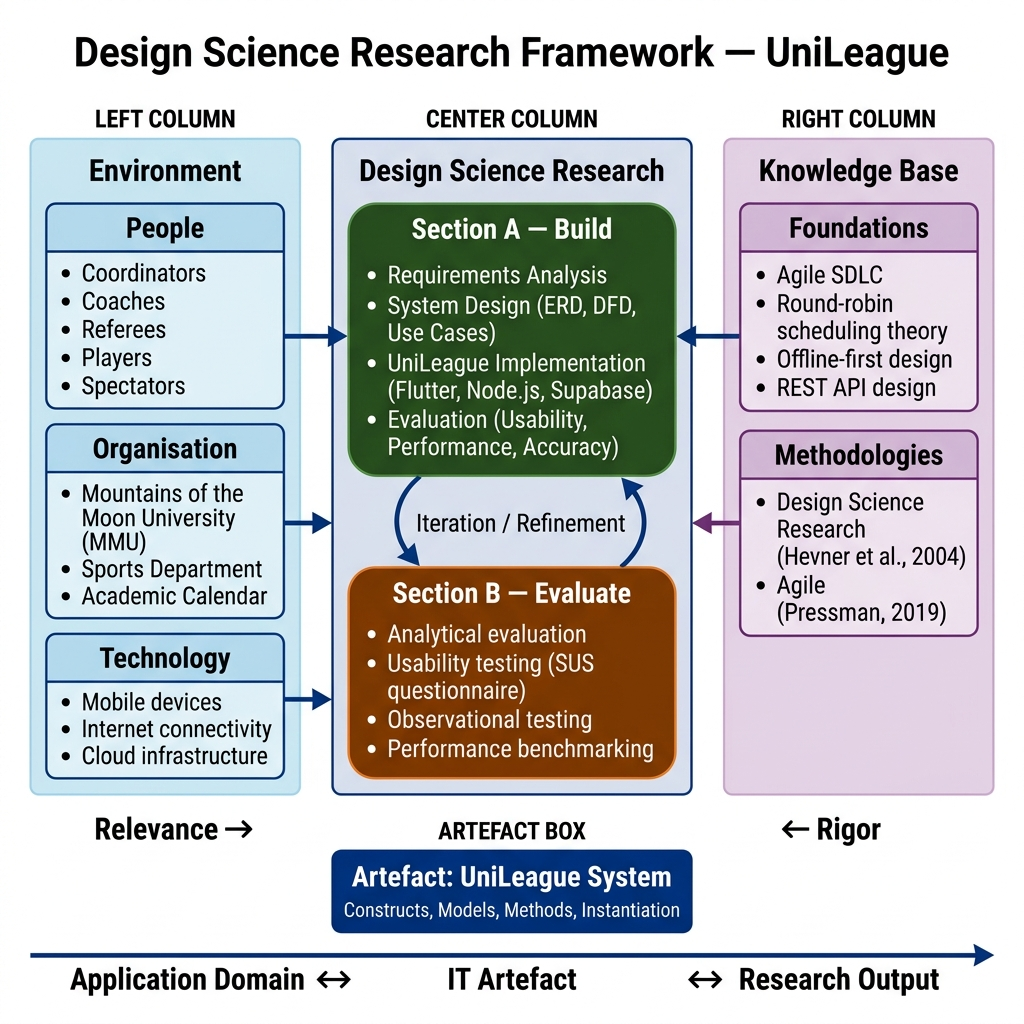
\includegraphics[width=0.80\linewidth]{dsr_framework.png}
\caption{Design Science Research Framework Applied to UniLeague}
\label{fig:dsr}
\end{figure}

\section{Study Population}
The study population consisted of stakeholders involved in soccer league activities at MMU,
including league administrators, coordinators, coaches, team captains, players, referees,
and spectators.

\begin{table}[H]
\centering
\caption{Study Population}
\begin{tabular}{p{5cm}p{3cm}p{6cm}}
\toprule
\textbf{Category} & \textbf{Estimated No.} & \textbf{Role in the Study}\\
\midrule
Sports coordinators & 2 & League administration and reporting.\\
Coaches and team captains & 10 & Team management and fixture coordination.\\
Players & 40 & Registration, fixtures, and performance tracking.\\
Referees & 6 & Match event recording and result submission.\\
Spectators and students & 30 & Access to fixtures, standings, and updates.\\
\textbf{Total} & \textbf{88} & \textbf{Representative soccer league stakeholders.}\\
\bottomrule
\end{tabular}
\end{table}

\section{Sampling Techniques}
The study used census sampling, purposive sampling, and simple random sampling. Census
sampling was used for league administrators and coordinators because the population was
small and all members were accessible. Purposive sampling was used to select coaches,
captains, and referees because they possess specific knowledge about soccer league
management. Simple random sampling was used to select players and spectators to obtain
diverse views from regular system users.

\section{Sample Size}
A sample size of 50 respondents was selected from the target population.

\begin{table}[H]
\centering
\caption{Sample Size Distribution}
\begin{tabular}{p{5cm}p{4cm}p{5cm}}
\toprule
\textbf{Category} & \textbf{Sample Size} & \textbf{Sampling Method}\\
\midrule
Sports coordinators & 2 & Census sampling\\
Coaches and team captains & 8 & Purposive sampling\\
Players & 20 & Simple random sampling\\
Referees & 5 & Purposive sampling\\
Spectators and students & 15 & Simple random sampling\\
\textbf{Total} & \textbf{50} & \textbf{Mixed sampling}\\
\bottomrule
\end{tabular}
\end{table}

\section{Data Collection Methods}
\subsection{Semi-Structured Interviews}
Interviews were conducted with sports coordinators, coaches, captains, and referees to identify
current workflows, pain points, and expectations for the proposed system.

\subsection{Questionnaires}
Questionnaires were administered to players and spectators to collect information about their
experiences with current soccer league communication and their expectations for a digital platform.

\subsection{Observation}
Observation was used to understand how league activities were coordinated during registration,
fixture communication, and match reporting, helping identify delays and gaps in current procedures.

\subsection{Document Review}
Existing documents such as fixture lists, team registration forms, result sheets, and spreadsheet
records were reviewed to identify data that needed to be captured in UniLeague.

\subsection{Usability Testing}
Usability testing sessions were conducted after system development to determine whether users
could perform major tasks such as logging in, registering teams, viewing fixtures, recording
scores, and checking standings.

\section{Data Analysis Methods}
Qualitative data from interviews and observation was analysed using thematic analysis. Common
themes were identified including communication delays, data duplication, fixture conflicts,
result delays, and lack of performance tracking. Quantitative data from questionnaires and
usability testing was analysed using descriptive statistics such as frequencies, percentages,
and mean scores.

\section{System Development Methodology}
The project used Agile software development \cite{pressman2019}. Development was organised
into iterative sprints, each producing a working system increment for stakeholder review.

\begin{enumerate}
  \item Requirements analysis and planning.
  \item System design and prototyping.
  \item Database schema design and backend API implementation.
  \item Frontend mobile and web interface development.
  \item Real-time event handling and offline-first capabilities.
  \item Testing, deployment preparation, and user evaluation.
\end{enumerate}

\begin{figure}[H]
\centering
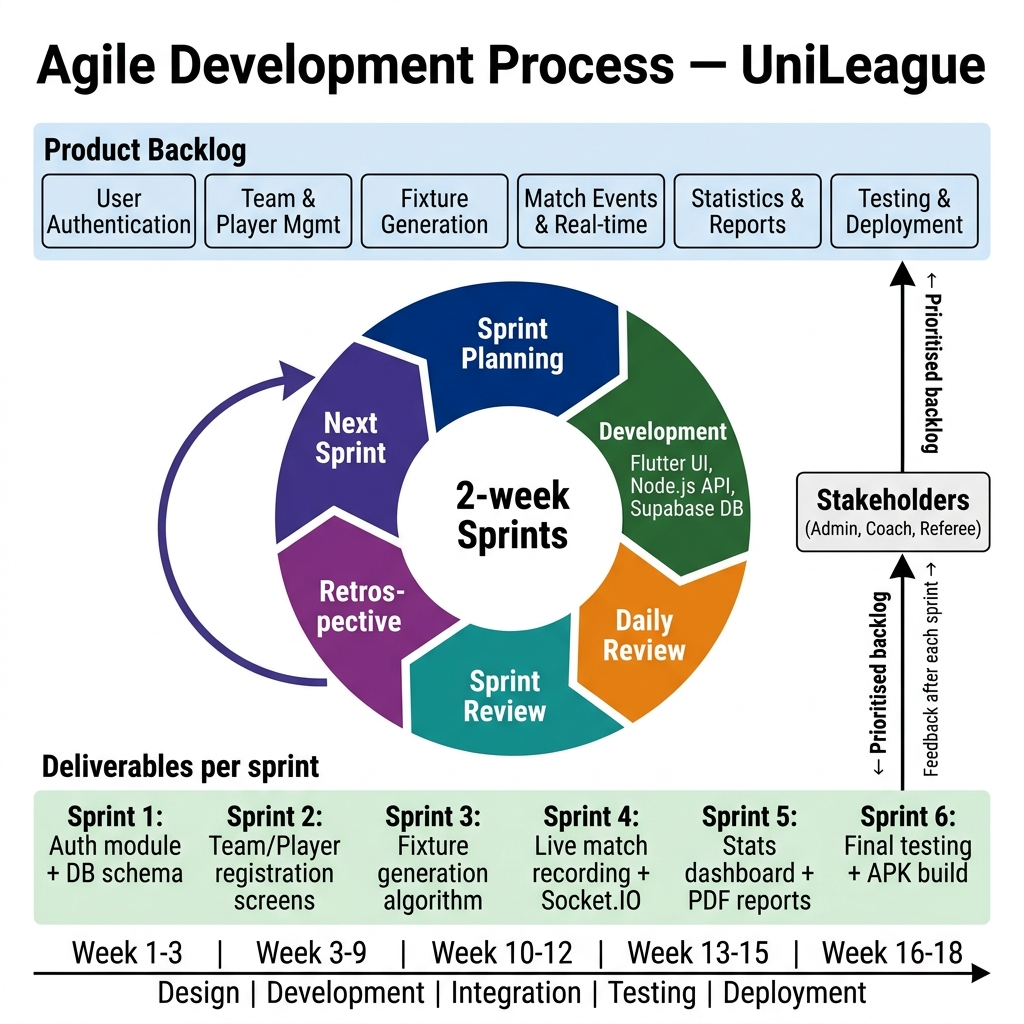
\includegraphics[width=0.80\linewidth]{agile_process.png}
\caption{Agile Development Process Used for UniLeague}
\label{fig:agile}
\end{figure}

\section{Tools and Technologies Used}
\begin{table}[H]
\centering
\caption{Development Tools and Technologies}
\begin{tabular}{p{4cm}p{4.5cm}p{5.5cm}}
\toprule
\textbf{Component} & \textbf{Technology} & \textbf{Purpose}\\
\midrule
Frontend & Flutter & Cross-platform mobile and web development.\\
State management & Provider & Application state across screens.\\
HTTP client & Dio & Frontend-to-backend API communication.\\
Backend & Node.js and Express & API development and business logic.\\
Database & Supabase PostgreSQL & Centralised league data storage.\\
ORM & Prisma & Structured database access and queries.\\
Authentication & Supabase Auth and JWT & Secure login and role-based access.\\
Real-time updates & Socket.IO & Live match updates and notifications.\\
Offline storage & SQLite via \texttt{sqflite} & Local data when internet is unavailable.\\
Connectivity & \texttt{connectivity\_plus} & Network status monitoring.\\
Charts & \texttt{fl\_chart} & Statistics and performance visualisations.\\
Reports & PDF and file saver tools & Generation and saving of league reports.\\
Security middleware & Helmet, CORS, Zod & Secure headers, CORS, and input validation.\\
Deployment & Docker & Containerisation and deployment.\\
Testing & \texttt{flutter\_test}, manual, UAT & Verification and validation.\\
\bottomrule
\end{tabular}
\end{table}

\section{Validity and Reliability}
Validity was ensured through triangulation of interviews, observations, questionnaires, and
document review. Research instruments were reviewed and piloted before full use. Stakeholder
feedback confirmed that identified problems and system requirements reflected real operational needs.

Reliability was supported through consistent interview guides, structured questionnaires,
documented testing procedures, and repeatable system test cases. Automated testing verified
the correctness of system modules. The System Usability Scale (SUS) was used to provide a
standardised usability measurement \cite{brooke1996}.

\section{Ethical Considerations}
Participants were informed about the purpose of the study and their participation was voluntary.
Consent was obtained before interviews, observations, and usability testing. Participant
responses were treated confidentially and used only for academic purposes. The system was
designed to protect user data through authentication, access control, and secure data storage.

\section{Limitations of the Study}
The study was limited by time, availability of respondents, and access to complete historical
league records. Some users had limited experience with digital sports systems, requiring
additional explanation during testing. Network reliability was also a limitation, leading to
the inclusion of offline storage support.

\section{Conclusion}
This chapter described the research and development methodology. It explained the DSR approach,
study population, sampling, data collection methods, data analysis, Agile development, tools,
validity, reliability, and ethical considerations. The next chapter presents system analysis
and design.

%% ========================================================
%% CHAPTER FOUR
%% ========================================================
\chapter{SYSTEM ANALYSIS AND DESIGN}
\section{Introduction}
This chapter presents the system analysis and design of UniLeague. It describes the existing
system and its limitations, the proposed system, user requirements, functional and non-functional
requirements, system architecture, process models, sequence diagrams, data flow design, and
database design.

\section{System Study}
\subsection{Current System}
The existing soccer league management process at MMU relies on manual and semi-digital tools.
Team and player registration is recorded on paper forms or spreadsheets. Fixtures are shared
through WhatsApp groups, noticeboards, or verbal communication. Match results are submitted
manually and later compiled by coordinators. League standings are updated manually and may
take several days after a match.

\subsection{Limitations of the Current System}
The major challenges identified through interviews, observation, and document review include:
\begin{enumerate}
  \item Delayed communication of fixtures, results, and announcements.
  \item Inconsistent and incomplete player and team registration records.
  \item Manual fixture preparation causing scheduling conflicts.
  \item Delayed league table updates after matches.
  \item Limited tracking of player performance statistics.
  \item Difficulty retrieving historical league records.
  \item Lack of real-time match updates for spectators.
  \item High administrative workload for sports coordinators.
  \item Substitution communication lacking audit trails.
\end{enumerate}

\subsection{Proposed System}
UniLeague is a cross-platform digital system designed to manage soccer league operations at MMU.
It provides a centralised platform for administrators, coaches, referees, players, and spectators
supporting team registration, player registration, fixture generation, match result recording,
match event recording, substitutions, standings, statistics, notifications, offline storage,
real-time updates, and report generation. Role-based access ensures users can only access
functions appropriate to their responsibilities.

\section{System Analysis}

\subsection{User Requirements}
\begin{table}[H]
\centering
\caption{System Users and Roles}
\begin{tabular}{p{4cm}p{10cm}}
\toprule
\textbf{User Role} & \textbf{Main Responsibilities}\\
\midrule
Administrator & Manages users, teams, players, fixtures, results, standings, reports, and system settings.\\
Sports Coordinator & Oversees league operations, verifies fixtures, monitors results, and generates reports.\\
Coach or Captain & Registers team details, manages player information, views fixtures and results.\\
Referee & Records match events, substitutions, cards, goals, and final scores.\\
Player & Views fixtures, results, standings, and personal performance information.\\
Spectator & Views public fixtures, results, standings, and match updates.\\
\bottomrule
\end{tabular}
\end{table}

\subsection{Functional Requirements}
\begin{table}[H]
\centering
\caption{Functional Requirements}
\begin{tabular}{p{2.5cm}p{11.5cm}}
\toprule
\textbf{ID} & \textbf{Description}\\
\midrule
FR01 & The system shall allow users to register and log in securely.\\
FR02 & The system shall support role-based access for all user types.\\
FR03 & The system shall allow administrators to create and manage teams.\\
FR04 & The system shall allow player registration and assignment to teams.\\
FR05 & The system shall generate and manage league fixtures using round-robin scheduling.\\
FR06 & The system shall allow referees to record match results.\\
FR07 & The system shall record match events such as goals, cards, and substitutions.\\
FR08 & The system shall automatically calculate and update league standings.\\
FR09 & The system shall display player and team performance statistics.\\
FR10 & The system shall send notifications and real-time match updates via Socket.IO.\\
FR11 & The system shall store selected data offline and synchronise when connectivity is restored.\\
FR12 & The system shall generate printable or downloadable PDF reports.\\
\bottomrule
\end{tabular}
\end{table}

\subsection{Non-Functional Requirements}
\begin{table}[H]
\centering
\caption{Non-Functional Requirements}
\begin{tabular}{p{3.5cm}p{10.5cm}}
\toprule
\textbf{Requirement} & \textbf{Description}\\
\midrule
Usability & Simple interface easy for students and non-technical staff to use.\\
Reliability & Data stored accurately; consistent league records maintained.\\
Security & User data protected through authentication, authorisation, validation, and access control.\\
Performance & System responds within acceptable time during normal use.\\
Scalability & Supports additional teams, players, and fixtures in future seasons.\\
Maintainability & Modular code and clear database structures for easier updates.\\
Portability & Runs on mobile and web platforms through Flutter.\\
Availability & Supports selected offline operations where internet is limited.\\
\bottomrule
\end{tabular}
\end{table}

\section{System Design}

\subsection{Architectural Design}
UniLeague uses a client-server architecture. The Flutter frontend provides user interfaces for
mobile and web users. The backend built with Node.js and Express processes requests, applies
business rules, and communicates with the database. Supabase PostgreSQL stores central data,
while SQLite stores selected local data for offline use. Socket.IO supports real-time updates
between the server and connected clients.

\begin{figure}[H]
\centering
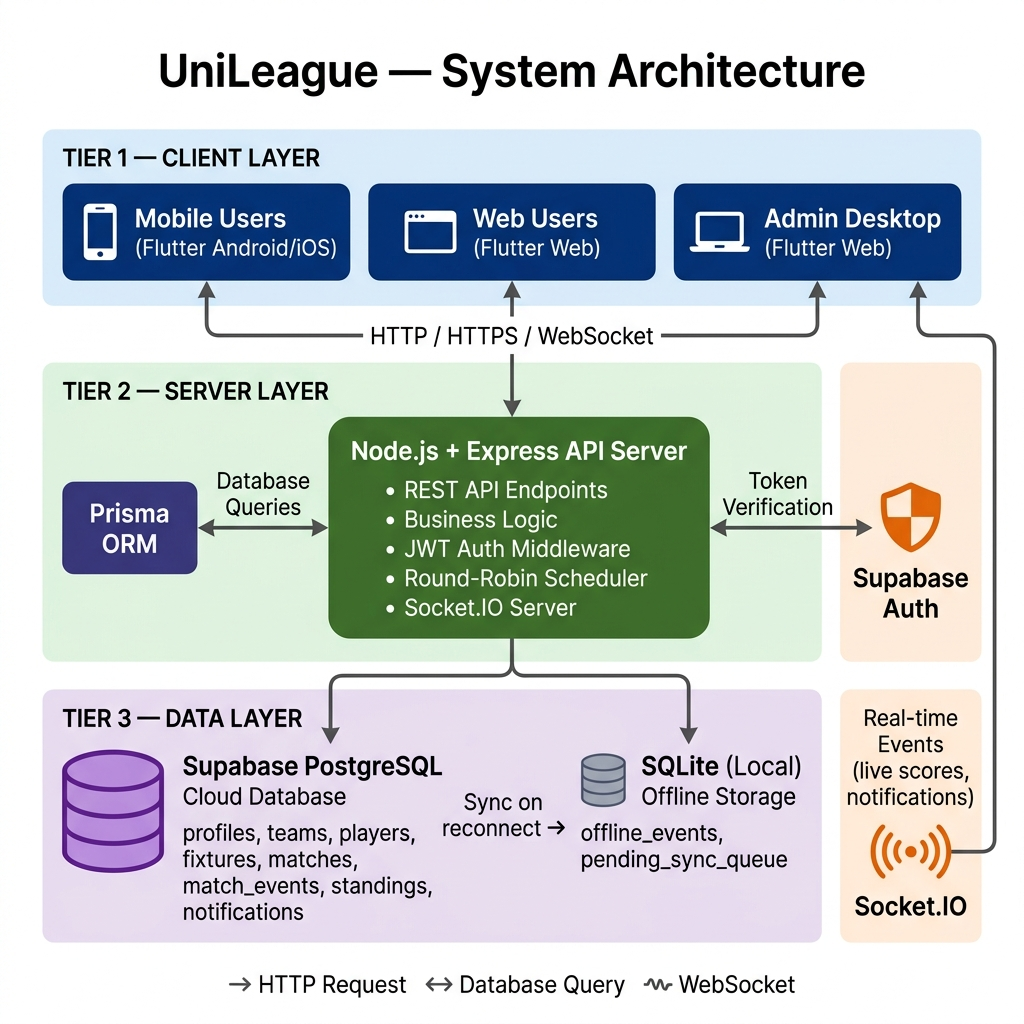
\includegraphics[width=0.80\linewidth]{system_architecture.png}
\caption{System Architecture of UniLeague}
\label{fig:architecture}
\end{figure}

\subsection{Process Modelling}
\subsubsection{Context Diagram}
The context diagram shows the interaction between UniLeague and its external entities including
coordinators, coaches, referees, players, and spectators. Data flows include team registrations,
fixture schedules, match results, performance statistics, and notifications.
\begin{figure}[H]
\centering
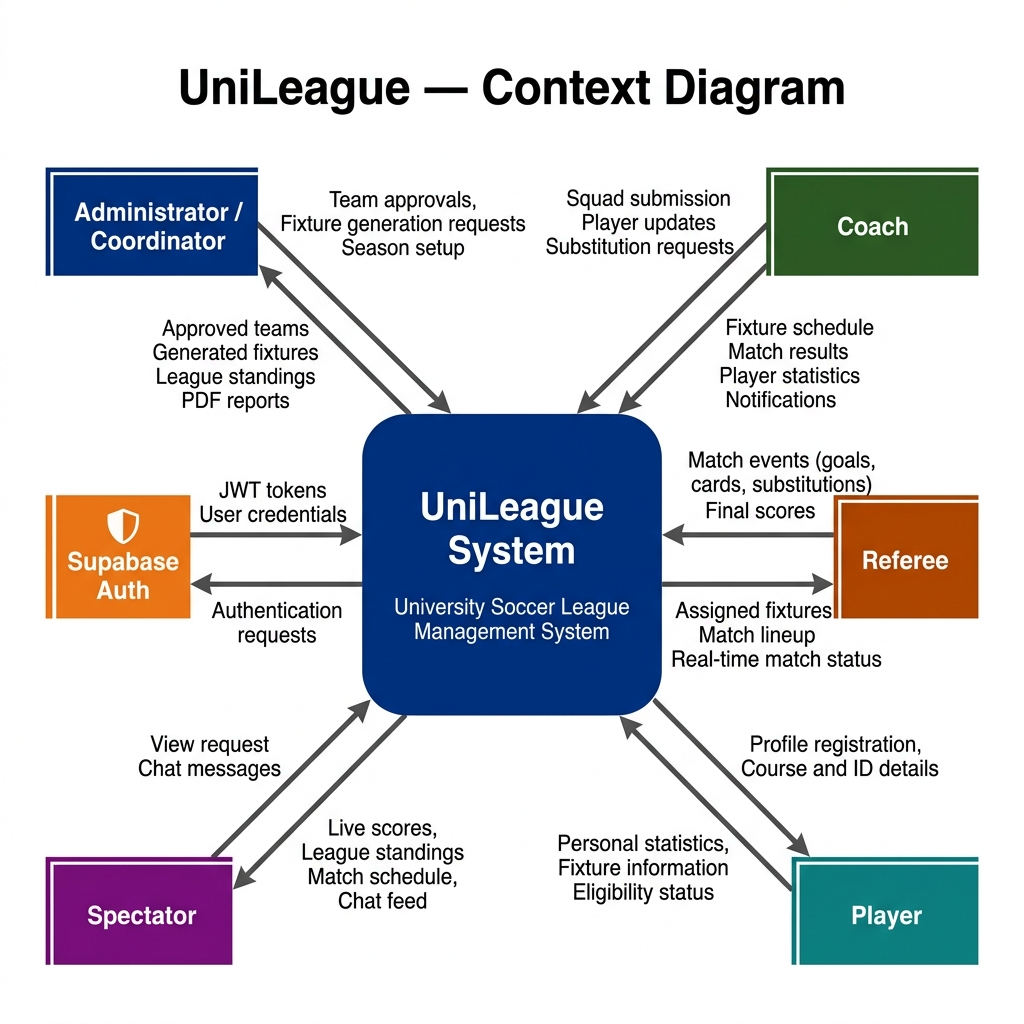
\includegraphics[width=0.80\linewidth]{context_diagram.png}
\caption{Context Diagram of UniLeague}
\label{fig:context}
\end{figure}

\subsubsection{Level-1 Data Flow Diagram}
The Level-1 DFD decomposes UniLeague into major processes: user authentication, team management,
fixture generation, match management, statistics computation, notification dispatch, and
report generation.
\begin{figure}[H]
\centering
\includegraphics[width=0.80\linewidth]{level1_dfd.png}
\caption{Level-1 Data Flow Diagram of UniLeague}
\label{fig:dfd}
\end{figure}

\subsubsection{Use Case Diagram}
The use case diagram shows how users interact with major system functions including login, team
registration, player management, fixture generation, result recording, event recording,
standings viewing, statistics viewing, notification management, and report generation.
\begin{figure}[H]
\centering
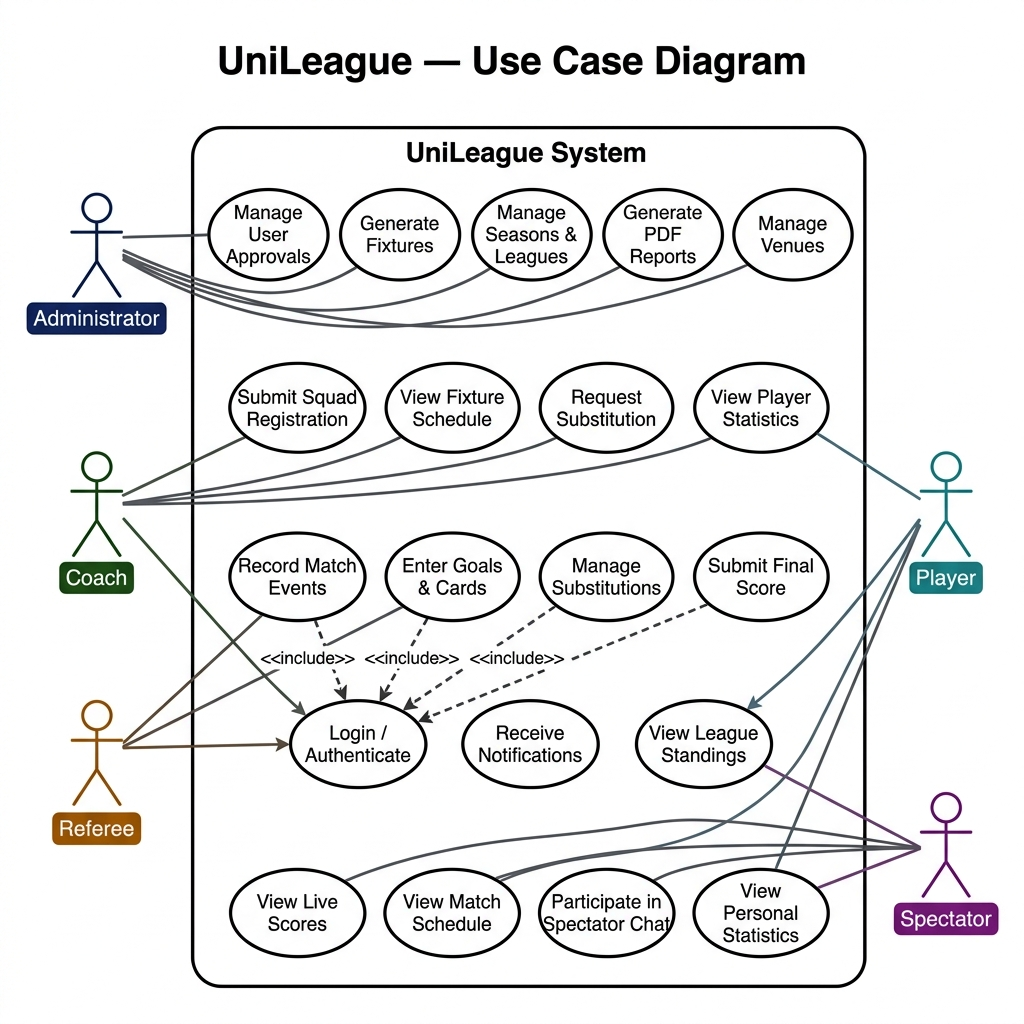
\includegraphics[width=0.80\linewidth]{use_case_diagram.png}
\caption{Use Case Diagram for UniLeague}
\label{fig:usecase}
\end{figure}

\subsection{Data Modelling}
\subsubsection{User Login Sequence}
The login sequence begins when a user enters credentials. The Flutter frontend sends a POST
request to the Node.js backend, which validates credentials against Supabase Auth. On success,
a JWT token is returned; the user is routed to their role-specific dashboard.
\begin{figure}[H]
\centering
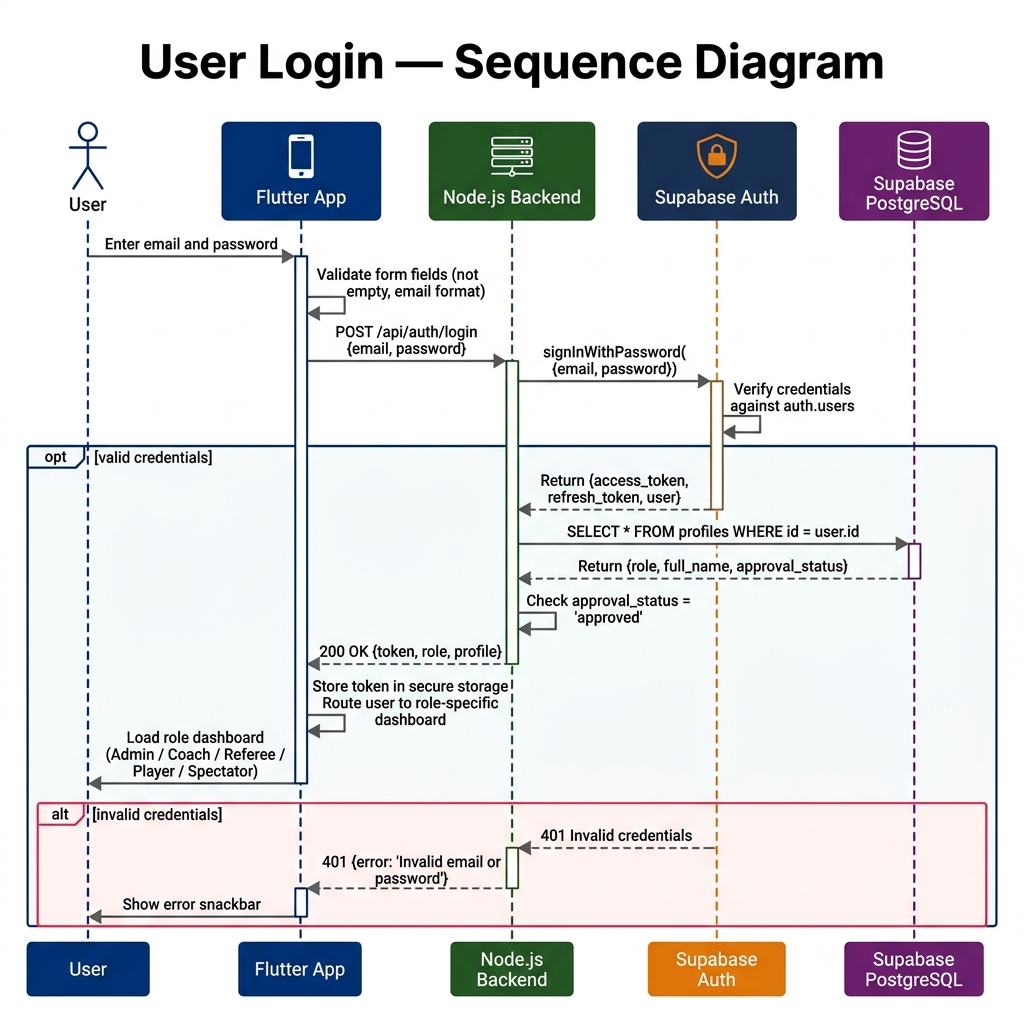
\includegraphics[width=0.80\linewidth]{seq_login.png}
\caption{Sequence Diagram: User Login}
\label{fig:seqlogin}
\end{figure}

\subsubsection{Fixture Generation Sequence}
The coordinator requests fixture generation. The backend retrieves registered teams, applies
the round-robin algorithm with conflict checking, stores generated fixtures in PostgreSQL via
Prisma, and returns the fixture list to the frontend.
\begin{figure}[H]
\centering
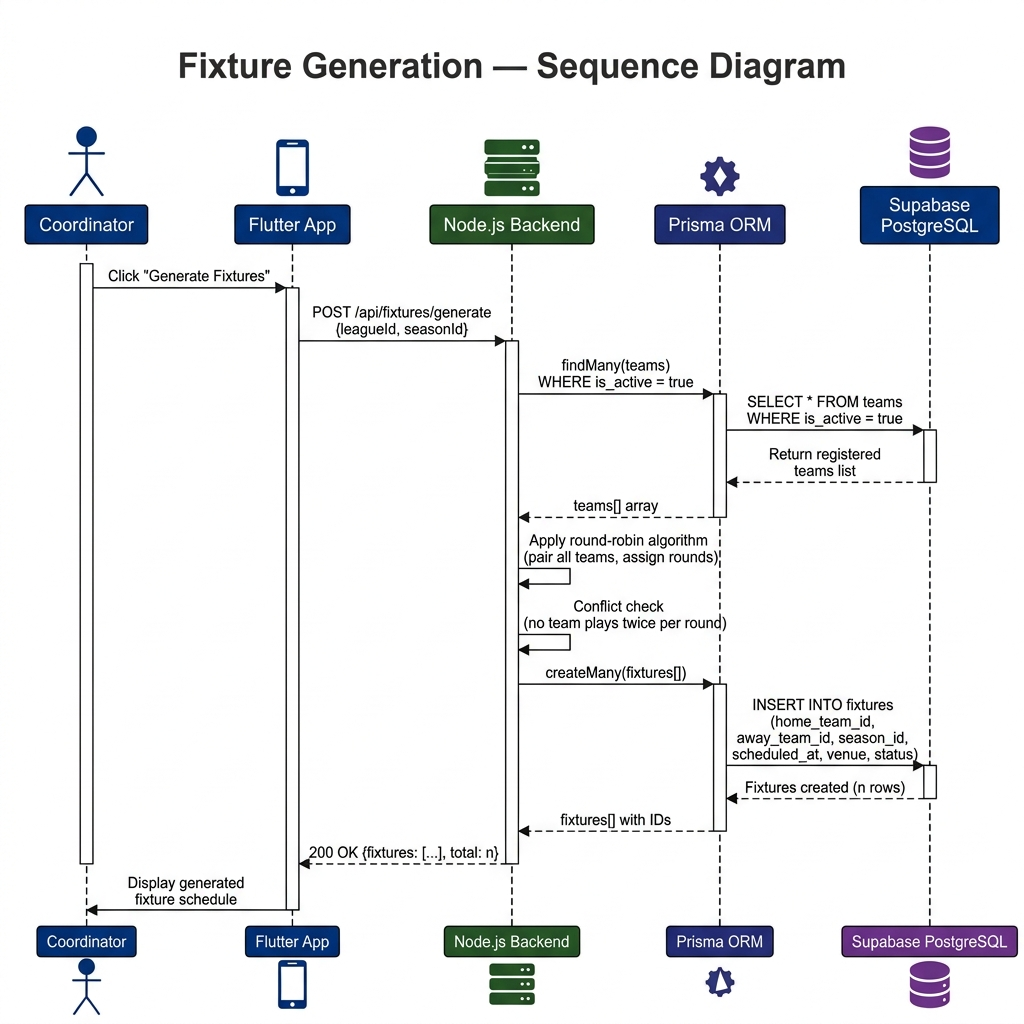
\includegraphics[width=0.80\linewidth]{seq_fixture.png}
\caption{Sequence Diagram: Fixture Generation}
\label{fig:seqfixture}
\end{figure}

\subsubsection{Match Event Recording Sequence}
The referee selects a live match and enters an event. The event is sent to the backend, stored
in the match\_events table, and broadcast via Socket.IO to all connected users in real time.
If offline, the event is saved to SQLite and synchronised when connectivity is restored.
\begin{figure}[H]
\centering
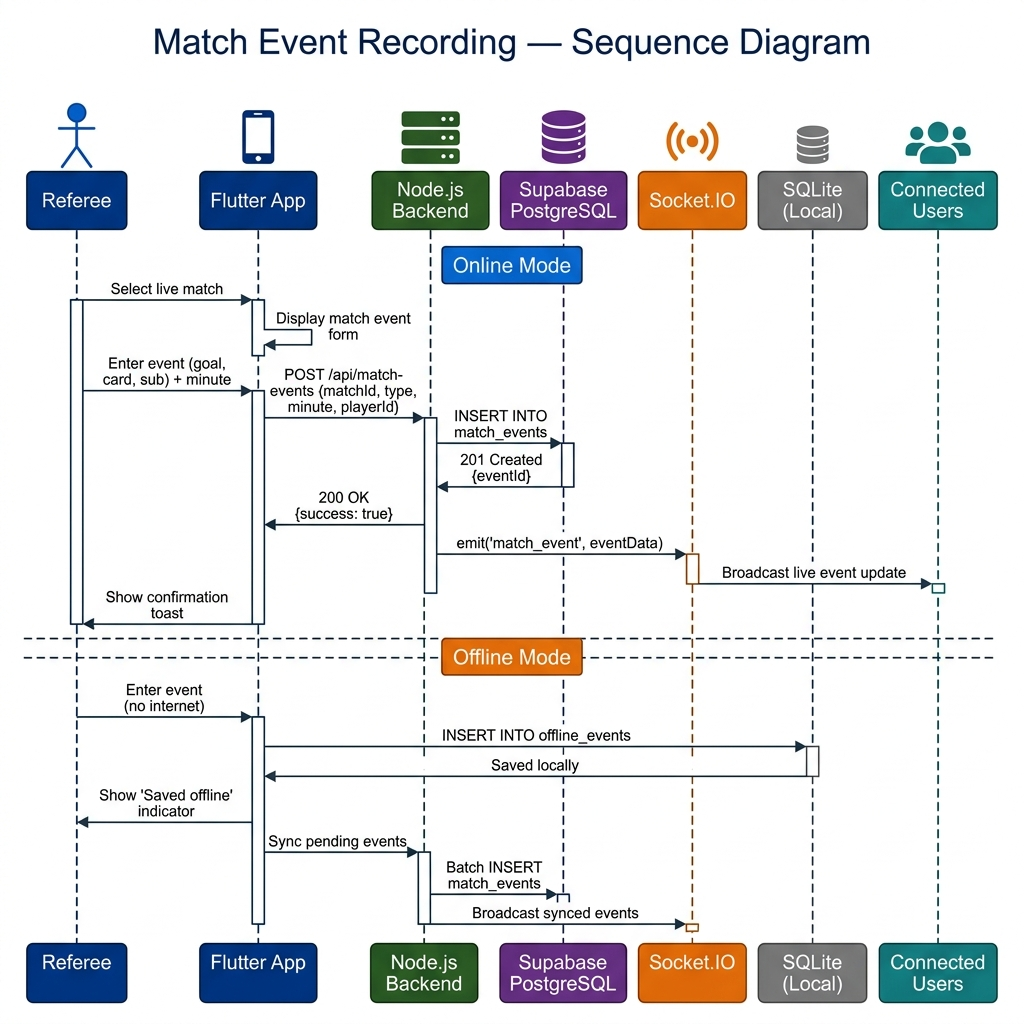
\includegraphics[width=0.80\linewidth]{seq_match_event.png}
\caption{Sequence Diagram: Match Event Recording}
\label{fig:seqevent}
\end{figure}

\subsection{Database Design}
The database was designed to store users, roles, teams, players, fixtures, matches, match events,
substitutions, standings, notifications, and audit records.

\begin{table}[H]
\centering
\caption{Main Database Entities}
\begin{tabular}{p{4cm}p{10cm}}
\toprule
\textbf{Entity} & \textbf{Description}\\
\midrule
Users & Stores user account information and authentication references.\\
Roles & Stores system roles (administrator, coach, referee, player, spectator).\\
Teams & Stores team details including name, coach, captain, and registration status.\\
Players & Stores player biodata, team assignment, position, and eligibility status.\\
Fixtures & Stores scheduled matches, dates, venues, and assigned teams.\\
Matches & Stores match status, scores, referee assignment, and result verification.\\
MatchEvents & Stores goals, cards, assists, fouls, and other match events.\\
Substitutions & Stores player substitution records with timestamps.\\
Standings & Stores computed league table data (points, wins, draws, losses, GD).\\
Notifications & Stores announcements and system messages.\\
AuditLogs & Stores traceable user actions for accountability.\\
\bottomrule
\end{tabular}
\end{table}

\begin{figure}[H]
\centering
\includegraphics[width=0.80\linewidth]{ERD.png}
\caption{Entity Relationship Diagram for UniLeague}
\label{fig:erd}
\end{figure}

\subsection{Core Database Tables}

The following tables represent the core database schema of UniLeague as implemented in
Supabase PostgreSQL. Each table shows the exact field names, PostgreSQL data types,
constraints, and descriptions as defined in the production database.
The symbol $\bigstar$ denotes a Primary Key and $\to$ denotes a Foreign Key reference.

%% ── public.profiles ────────────────────────────────────────────
\subsubsection{Profiles Table}
\begin{table}[H]
\centering
\caption{Database Table: \texttt{public.profiles}}
\setlength{\tabcolsep}{4pt}
\begin{tabular}{p{0.4cm}p{3.2cm}p{2.3cm}p{3.0cm}p{4.8cm}}
\rowcolor[HTML]{003087}
{\color{white}\textbf{\#}} &
{\color{white}\textbf{Field}} &
{\color{white}\textbf{Type}} &
{\color{white}\textbf{Constraints}} &
{\color{white}\textbf{Description}} \\
\rowcolor[HTML]{EEF2FF}
$\bigstar$ & id & uuid & PK, NOT NULL & Unique identifier; references auth.users(id) \\
\rowcolor[HTML]{FFFFFF}
 & full\_name & text & Nullable & Full legal name of the system user \\
\rowcolor[HTML]{EEF2FF}
 & email & text & Nullable & User email address for communication \\
\rowcolor[HTML]{FFFFFF}
 & phone & text & Nullable & User contact phone number \\
\rowcolor[HTML]{EEF2FF}
 & role & text & DEFAULT 'spectator' & System role: admin, coach, referee, player, or spectator \\
\rowcolor[HTML]{FFFFFF}
 & approval\_status & text & DEFAULT 'approved' & Account status: pending, approved, or rejected \\
\rowcolor[HTML]{EEF2FF}
 & avatar\_url & text & Nullable & URL to the user's profile photo stored in Supabase Storage \\
\rowcolor[HTML]{FFFFFF}
 & team\_name & text & Nullable & Team name linked to the user (used by coaches) \\
\rowcolor[HTML]{EEF2FF}
 & created\_at & timestamptz & NOT NULL, DEFAULT now() & Timestamp when the profile record was created \\
\rowcolor[HTML]{FFFFFF}
 & updated\_at & timestamptz & NOT NULL, DEFAULT now() & Timestamp when the profile was last updated \\
\end{tabular}
\end{table}

%% ── public.teams ───────────────────────────────────────────────
\subsubsection{Teams Table}
\begin{table}[htbp]
\centering
\caption{Database Table: \texttt{public.teams}}
\setlength{\tabcolsep}{4pt}
\begin{tabular}{p{0.4cm}p{3.5cm}p{2.3cm}p{3.0cm}p{4.5cm}}
\rowcolor[HTML]{003087}
{\color{white}\textbf{\#}} &
{\color{white}\textbf{Field}} &
{\color{white}\textbf{Type}} &
{\color{white}\textbf{Constraints}} &
{\color{white}\textbf{Description}} \\
\rowcolor[HTML]{EEF2FF}
$\bigstar$ & id & uuid & PK, NOT NULL & Auto-generated unique team identifier \\
\rowcolor[HTML]{FFFFFF}
 & name & text & NOT NULL, UNIQUE & Official registered name of the team \\
\rowcolor[HTML]{EEF2FF}
$\to$ & coach\_id & uuid & NOT NULL, UNIQUE, FK & References profiles(id); one coach per team \\
\rowcolor[HTML]{FFFFFF}
 & logo\_url & text & Nullable & URL to the team badge or logo image \\
\rowcolor[HTML]{EEF2FF}
 & home\_color & text & Nullable & Team home jersey colour code \\
\rowcolor[HTML]{FFFFFF}
 & away\_color & text & Nullable & Team away jersey colour code \\
\rowcolor[HTML]{EEF2FF}
 & is\_active & boolean & NOT NULL, DEFAULT true & Whether the team is active in the current season \\
\rowcolor[HTML]{FFFFFF}
 & submission\_status & text & NOT NULL, DEFAULT 'draft' & Squad status: draft, submitted, approved, or rejected \\
\rowcolor[HTML]{EEF2FF}
 & submitted\_at & timestamptz & Nullable & Timestamp when squad was submitted for admin approval \\
\rowcolor[HTML]{FFFFFF}
 & created\_at & timestamptz & NOT NULL, DEFAULT now() & Timestamp when the team record was created \\
\end{tabular}
\end{table}
\vspace{4pt}

%% ── public.players ─────────────────────────────────────────────
\subsubsection{Players Table}
\setlength{\tabcolsep}{4pt}
\begin{longtable}{p{0.4cm}p{3.5cm}p{2.3cm}p{3.0cm}p{4.5cm}}
\caption{Database Table: \texttt{public.players}}\\
\rowcolor[HTML]{003087}
{\color{white}\textbf{\#}} &
{\color{white}\textbf{Field}} &
{\color{white}\textbf{Type}} &
{\color{white}\textbf{Constraints}} &
{\color{white}\textbf{Description}} \\
\endfirsthead
\rowcolor[HTML]{003087}
{\color{white}\textbf{\#}} &
{\color{white}\textbf{Field}} &
{\color{white}\textbf{Type}} &
{\color{white}\textbf{Constraints}} &
{\color{white}\textbf{Description}} \\
\endhead
\rowcolor[HTML]{EEF2FF}
$\bigstar$ & id & uuid & PK, NOT NULL & Auto-generated unique player identifier \\
\rowcolor[HTML]{FFFFFF}
$\to$ & team\_id & uuid & NOT NULL, FK & References teams(id); the player's registered team \\
\rowcolor[HTML]{EEF2FF}
 & full\_name & text & NOT NULL & Player's full legal name \\
\rowcolor[HTML]{FFFFFF}
 & jersey\_number & integer & NOT NULL & Player's shirt number within the team \\
\rowcolor[HTML]{EEF2FF}
 & position & text & CHECK (GK, DEF, MID, FWD) & Player's primary field position \\
\rowcolor[HTML]{FFFFFF}
 & date\_of\_birth & date & Nullable & Player's date of birth for age eligibility checks \\
\rowcolor[HTML]{EEF2FF}
 & reg\_no & text & Nullable & University student registration number \\
\rowcolor[HTML]{FFFFFF}
 & university\_id & text & Nullable & University student identity card number \\
\rowcolor[HTML]{EEF2FF}
 & course & text & Nullable & Academic programme the player is enrolled in \\
\rowcolor[HTML]{FFFFFF}
 & year\_of\_study & text & Nullable & Current year of academic study \\
\rowcolor[HTML]{EEF2FF}
 & is\_eligible & boolean & NOT NULL, DEFAULT true & Whether the player is cleared to participate in matches \\
\rowcolor[HTML]{FFFFFF}
 & goals & integer & NOT NULL, DEFAULT 0 & Total goals scored by the player this season \\
\rowcolor[HTML]{EEF2FF}
 & assists & integer & NOT NULL, DEFAULT 0 & Total goal assists by the player this season \\
\rowcolor[HTML]{FFFFFF}
 & yellow\_cards & integer & NOT NULL, DEFAULT 0 & Total yellow cards received this season \\
\rowcolor[HTML]{EEF2FF}
 & red\_cards & integer & NOT NULL, DEFAULT 0 & Total red cards received this season \\
\rowcolor[HTML]{FFFFFF}
 & matches\_played & integer & NOT NULL, DEFAULT 0 & Total number of matches the player appeared in \\
\end{longtable}

%% ── public.fixtures ────────────────────────────────────────────
\subsubsection{Fixtures Table}
\begin{table}[htbp]
\centering
\caption{Database Table: \texttt{public.fixtures}}
\setlength{\tabcolsep}{4pt}
\begin{tabular}{p{0.4cm}p{3.5cm}p{2.3cm}p{3.0cm}p{4.5cm}}
\rowcolor[HTML]{003087}
{\color{white}\textbf{\#}} &
{\color{white}\textbf{Field}} &
{\color{white}\textbf{Type}} &
{\color{white}\textbf{Constraints}} &
{\color{white}\textbf{Description}} \\
\rowcolor[HTML]{EEF2FF}
$\bigstar$ & id & uuid & PK, NOT NULL & Auto-generated unique fixture identifier \\
\rowcolor[HTML]{FFFFFF}
$\to$ & season\_id & uuid & NOT NULL, FK & References seasons(id); the season this fixture belongs to \\
\rowcolor[HTML]{EEF2FF}
$\to$ & home\_team\_id & uuid & NOT NULL, FK & References teams(id); the home team for this fixture \\
\rowcolor[HTML]{FFFFFF}
$\to$ & away\_team\_id & uuid & NOT NULL, FK & References teams(id); the away team for this fixture \\
\rowcolor[HTML]{EEF2FF}
$\to$ & referee\_id & uuid & Nullable, FK & References profiles(id); the assigned match referee \\
\rowcolor[HTML]{FFFFFF}
 & scheduled\_at & timestamptz & NOT NULL & Date and time the match is scheduled to take place \\
\rowcolor[HTML]{EEF2FF}
 & venue & text & Nullable & Name of the venue where the match will be played \\
\rowcolor[HTML]{FFFFFF}
 & status & text & NOT NULL, DEFAULT 'scheduled' & Fixture status: scheduled, postponed, cancelled, completed \\
\rowcolor[HTML]{EEF2FF}
 & created\_at & timestamptz & NOT NULL, DEFAULT now() & Timestamp when the fixture record was created \\
\end{tabular}
\end{table}

%% ── public.match_events ────────────────────────────────────────
\subsubsection{Match Events Table}
\begin{table}[H]
\centering
\caption{Database Table: \texttt{public.match\_events}}
\setlength{\tabcolsep}{4pt}
\begin{tabular}{p{0.4cm}p{3.5cm}p{2.3cm}p{3.0cm}p{4.5cm}}
\rowcolor[HTML]{003087}
{\color{white}\textbf{\#}} &
{\color{white}\textbf{Field}} &
{\color{white}\textbf{Type}} &
{\color{white}\textbf{Constraints}} &
{\color{white}\textbf{Description}} \\
\rowcolor[HTML]{EEF2FF}
$\bigstar$ & id & uuid & PK, NOT NULL & Auto-generated unique match event identifier \\
\rowcolor[HTML]{FFFFFF}
$\to$ & match\_id & uuid & NOT NULL, FK & References matches(id); the match this event belongs to \\
\rowcolor[HTML]{EEF2FF}
$\to$ & team\_id & uuid & NOT NULL, FK & References teams(id); the team associated with the event \\
\rowcolor[HTML]{FFFFFF}
$\to$ & player\_id & uuid & Nullable, FK & References players(id); player who caused the event \\
\rowcolor[HTML]{EEF2FF}
 & event\_type & text & NOT NULL, CHECK & Type: goal, own\_goal, yellow\_card, red\_card, sub\_in, sub\_out \\
\rowcolor[HTML]{FFFFFF}
 & minute & integer & NOT NULL, CHECK (0--120) & Match minute when the event occurred \\
\rowcolor[HTML]{EEF2FF}
 & notes & text & Nullable & Additional referee notes or comments about the event \\
\rowcolor[HTML]{FFFFFF}
 & created\_at & timestamptz & NOT NULL, DEFAULT now() & Timestamp when the event record was saved to the database \\
\end{tabular}
\end{table}

\section{Conclusion}
This chapter presented the analysis and design of UniLeague. It described the weaknesses of
the existing system, proposed system features, system users, requirements, architecture,
process models, sequence diagrams, data flow, and database structure. These design outputs
provided the foundation for the implementation discussed in Chapter Five.

%% ========================================================
%% CHAPTER FIVE
%% ========================================================
\chapter{SYSTEM IMPLEMENTATION, TESTING AND EVALUATION}
\section{Introduction}
This chapter presents the implementation, testing, and evaluation of UniLeague. It explains
how the designed system was developed, the major modules implemented, the user interfaces
created, the testing approaches used to validate the system, and the challenges encountered.

\section{Implementation Plan}
The system was implemented over eighteen weeks using Agile development, with each sprint
producing a working component reviewed and improved based on stakeholder feedback.

\begin{table}[H]
\centering
\caption{Implementation Plan Summary}
\begin{tabular}{p{4cm}p{3cm}p{7cm}}
\toprule
\textbf{Phase} & \textbf{Weeks} & \textbf{Deliverables}\\
\midrule
Requirements and Design & 1--3 & Requirements, prototypes, database design, architecture\\
Backend and Database & 3--9 & API, authentication, PostgreSQL schema, core logic\\
Frontend Development & 3--9 & Flutter mobile and web interfaces\\
Integration and Real-Time & 10--12 & WebSocket updates, synchronisation, offline support\\
Testing and Refinement & 13--15 & Unit testing, usability testing, bug fixes\\
Deployment and Evaluation & 16--18 & Deployment, user training, pilot evaluation, reporting\\
\bottomrule
\end{tabular}
\end{table}

\section{System Development}
This section describes the major technical components implemented during the development
of UniLeague, covering the frontend, backend, database, offline storage, and real-time modules.

\subsection{Implementation Overview}
UniLeague was implemented as a cross-platform client-server system. The frontend was developed
using Flutter, while the backend was implemented using Node.js and Express. Supabase PostgreSQL
provided centralised database services and authentication support. Prisma was used to simplify
interaction with the PostgreSQL database, and Socket.IO enabled real-time match updates.

\subsection{Frontend Implementation}
The frontend was implemented using Flutter \cite{flutter2024}. Provider was used for state
management, while Dio was used for communication with backend APIs. The frontend includes
offline support using \texttt{sqflite} and connectivity detection through \texttt{connectivity\_plus}.

\subsection{Backend Implementation}
The backend was implemented using Node.js and Express, providing RESTful API endpoints for
authentication, teams, players, fixtures, matches, events, standings, statistics, and reports.
Prisma was used to interact with the PostgreSQL database \cite{prisma2024}. The backend
validates incoming data using Zod and protects API access through JWT-based authorisation
and role checks. Helmet and CORS settings were applied to improve API security \cite{helmet2024}.

\subsection{Database Implementation}
Supabase PostgreSQL was used as the main database \cite{supabase2024}. The database stores
structured league data and supports secure access through authentication and row-level security.
Tables were designed with relational integrity ensuring consistency between users, teams, players,
fixtures, matches, and events.

\subsection{Offline Implementation}
Offline support was implemented using SQLite through \texttt{sqflite}. Selected data such as
fixtures and match events can be stored locally when the device has no internet connection.
When connectivity is restored, the application synchronises local data with the central database.

\subsection{Real-Time Updates}
Socket.IO was used to support real-time updates \cite{socketio2024}. When match events are
recorded, updates are pushed immediately to all connected users, allowing spectators, players,
and coordinators to receive timely match information without refreshing the application.

\subsection{Reporting and Statistics}
The system computes league standings based on match results. Statistics include goals scored,
goals conceded, goal difference, points, top scorers, cards, and match history. Charts are
displayed using \texttt{fl\_chart}, while reports can be generated in PDF format.

\section{System Integration}
System integration involved connecting the Flutter frontend to the Node.js backend APIs,
linking the backend to Supabase PostgreSQL, enabling SQLite offline storage, and configuring
Socket.IO for real-time WebSocket communication. The integration ensured that when a referee
submits a match event offline, it is saved locally and then synchronised to the central
database once connectivity is restored, which subsequently triggers a real-time WebSocket
broadcast to update the standings and live scores on all connected spectator devices.

\section{System Interfaces}
The user interface was designed to be clean, responsive, and accessible on both mobile devices
and web browsers, built with Flutter following Material Design principles.

\subsection{Login Screen}
The login screen is the secure entry point. Coordinators and referees authenticate with a
registered e-mail address and password; the system routes each user to the appropriate
interface based on their assigned role.
\begin{figure}[H]\centering
\includegraphics[width=0.55\linewidth]{login.jpg}
\caption{User Login and Authentication Screen}\label{fig:login}
\end{figure}

\subsection{Administrator Dashboard}
The administrator dashboard provides a high-level summary of the active season --- total
registered teams, players, scheduled fixtures, and completed matches --- alongside
quick-action buttons for the most common tasks.
\begin{figure}[H]\centering
\includegraphics[width=0.8\linewidth,height=0.4\textheight]{admin_dashboard.png}
\caption{Administrator Dashboard Overview}\label{fig:dashboard}
\end{figure}

\subsection{Team and Player Management}
The team management screen allows the coordinator to register, view, and edit all participating
clubs. Each entry shows the team name, head coach, squad size, and current points total.
\begin{figure}[H]\centering
\includegraphics[width=0.55\linewidth]{team_management.png}
\caption{Team and Player Management Screen}\label{fig:teams}
\end{figure}

\subsection{Fixture Management}
The fixture management screen displays the complete match schedule for the season. Matches are
filterable by status (\textit{Scheduled}, \textit{Live}, or \textit{Completed}).
\begin{figure}[H]\centering
\includegraphics[width=0.55\linewidth]{fixture.png}
\caption{Fixture Generation and Schedule Screen}\label{fig:fixtures}
\end{figure}

\subsection{Match Event Recording}
The match event recording screen is the referee's primary interface during live matches. It
displays the running score and match timer, and accepts real-time entry of goals, yellow cards,
red cards, and substitutions. A synchronisation indicator shows whether events are being saved
to the server or stored locally pending reconnection.
\begin{figure}[H]\centering
\includegraphics[width=0.55\linewidth]{match_record.jpg}
\caption{Match Event Recording Screen (Referee Interface)}\label{fig:recording}
\end{figure}

\subsection{League Standings}
The standings screen presents the automatically computed points table, ranked by points with
goal difference and goals scored as tiebreakers.
\begin{figure}[H]\centering
\includegraphics[width=0.55\linewidth]{standings.jpg}
\caption{Live League Standings Table}\label{fig:standings}
\end{figure}

\subsection{Player Statistics}
The statistics screen provides performance analytics for players and teams. The top-scorers
bar chart, rendered with \texttt{fl\_chart}, compares goal tallies across all players.
\begin{figure}[H]\centering
\includegraphics[width=0.55\linewidth]{statistics.png}
\caption{Performance Analytics and Player Statistics Screen}\label{fig:statistics}
\end{figure}

\subsection{Generated Administrative Report}
The system produces formatted PDF reports. The coordinator selects the report type and
previews the output before downloading.
\begin{figure}[H]\centering
\includegraphics[width=0.55\linewidth]{pdf_report.png}
\caption{Generated Administrative Report (PDF Preview)}\label{fig:report}
\end{figure}

\section{Fixture Generation Logic}
The fixture generation module creates match pairings using a round-robin algorithm. Each team
is scheduled to play against every other team. If the number of teams is odd, a bye is
introduced so one team rests in each round. The module checks for basic scheduling constraints
such as avoiding the same team appearing in two fixtures simultaneously. Administrators can
review and adjust generated fixtures before publishing.

\section{Standings Calculation}
League standings are calculated using standard soccer rules. A team receives three points for
a win, one point for a draw, and zero for a loss.

$$\text{Goal Difference} = \text{Goals For} - \text{Goals Against}$$
$$\text{Points} = (3 \times \text{Wins}) + (1 \times \text{Draws})$$

The league table is ranked using points, goal difference, goals scored, and administrative
tie-breakers where necessary.

\section{Testing Strategy}
Testing was conducted to verify whether the system met functional and non-functional
requirements \cite{pressman2019}. The testing approach included unit testing, widget testing,
integration testing, manual functional testing, usability testing, and user acceptance testing.

\subsection{Unit and Widget Testing}
Flutter unit and widget tests verified selected application logic and user interface components,
confirming that individual widgets and functions behaved as expected.

\subsection{Integration Testing}
Integration testing verified that the frontend, backend, and database worked together correctly,
testing processes such as login, team registration, fixture retrieval, result submission, and
standings calculation.

\subsection{Manual Functional Testing}
\begin{table}[H]
\centering
\caption{Functional Test Results}
\begin{tabular}{p{3.5cm}p{4.5cm}p{3.5cm}p{2cm}}
\toprule
\textbf{Test Case} & \textbf{Expected Result} & \textbf{Actual Result} & \textbf{Status}\\
\midrule
User login & Valid users access dashboard & Role-based dashboard loaded & Passed\\
Team registration & Admin creates new team & Team created and saved & Passed\\
Player registration & Player assigned to team & Record saved under team & Passed\\
Fixture creation & Fixtures generated and listed & Fixtures displayed & Passed\\
Result entry & Referee submits final score & Score saved, match completed & Passed\\
Standings update & Table updates after result & Standings recalculated & Passed\\
Offline event storage & Event stored locally offline & Saved in local SQLite & Passed\\
Real-time update & Connected users get update & Update appeared instantly & Passed\\
Report generation & Admin generates PDF report & PDF report downloaded & Passed\\
\bottomrule
\end{tabular}
\end{table}

\subsection{Usability Testing}
\begin{table}[H]
\centering
\caption{Usability Evaluation Summary}
\begin{tabular}{p{6cm}p{4cm}p{4cm}}
\toprule
\textbf{Evaluation Item} & \textbf{Positive Responses} & \textbf{Interpretation}\\
\midrule
Ease of login and navigation & 88\% & Most users found navigation easy.\\
Clarity of fixture information & 92\% & Fixtures were easy to understand.\\
Ease of result recording & 84\% & Referees found the interface useful.\\
Usefulness of standings & 94\% & Users valued automatic table updates.\\
Overall satisfaction & 90\% & Most users were satisfied.\\
\bottomrule
\end{tabular}
\end{table}

\subsection{User Acceptance Testing}
\begin{table}[H]
\centering
\caption{User Acceptance Testing Mean Scores (Scale: 1--5)}
\begin{tabular}{p{4.5cm}p{3cm}p{3cm}p{3cm}}
\toprule
\textbf{User Group} & \textbf{Ease of Use} & \textbf{Usefulness} & \textbf{Satisfaction}\\
\midrule
Coordinators & 4.4 & 4.6 & 4.5\\
Coaches & 4.2 & 4.5 & 4.4\\
Referees & 4.3 & 4.5 & 4.4\\
Players / Spectators & 4.1 & 4.3 & 4.2\\
\textbf{Overall Average} & \textbf{4.25} & \textbf{4.48} & \textbf{4.38}\\
\bottomrule
\end{tabular}
\end{table}

\section{System Validation and Evaluation}

\subsection{System Validation}
System validation confirmed that UniLeague met the stated requirements and stakeholder
expectations. Validation was conducted by asking representative users to perform real-world
tasks --- team registration, fixture generation, match event recording, and standings viewing
--- and confirming that the system produced correct and expected results. All four specific
objectives were verified through structured test cases and stakeholder confirmation sessions.

\subsection{System Evaluation}
The evaluation showed that UniLeague improved several aspects of soccer league management at
MMU. It centralised team and player records, reduced dependence on scattered communication
channels, improved fixture visibility, supported faster result processing, and provided
automatic standings. Users appreciated mobile access to fixtures and standings. Referees and
coordinators found match event recording useful for improving accuracy.

\section{Challenges and Solutions}
\subsection{Limited Internet Connectivity}
Some users experienced unreliable internet connectivity at match venues. This was addressed
through SQLite offline storage and automatic synchronisation when connectivity was restored.

\subsection{Different Levels of Digital Literacy}
Some stakeholders were not familiar with digital systems. This was addressed through simplified
interface design, clear labels, in-app help text, and user training sessions.

\subsection{Fixture Constraint Complexity}
Fixture generation required consideration of teams, venues, and time slots. This was addressed
by extending the round-robin algorithm with basic conflict detection that flags duplicate team
or venue assignments.

\subsection{Device Variation}
Users accessed the system from different Android phones, tablets, and web browsers. Flutter
was used to support consistent cross-platform access with responsive layouts.

\section{Discussion of Findings}
The findings indicate that a cross-platform system can improve university soccer league
management when designed around local workflows \cite{sarlak2024}. UniLeague addressed key
limitations of the existing system by integrating registration, fixtures, match recording,
standings, statistics, and communication into one platform. The use of Flutter supported
access across devices, while Supabase PostgreSQL provided centralised storage. Offline local
storage addressed connectivity challenges, and real-time updates improved communication.

\section{Conclusion}
This chapter presented the implementation, testing, and evaluation of UniLeague. It described
the frontend, backend, database, offline storage, real-time updates, reporting, user interfaces,
fixture generation, standings calculation, testing results, challenges, and evaluation findings.

%% ========================================================
%% CHAPTER SIX
%% ========================================================
\chapter{RESULTS, CONCLUSIONS AND RECOMMENDATIONS}
\section{Introduction}
This chapter presents the results, discussion, conclusions, contributions, recommendations,
limitations, and areas for future research based on the development and evaluation of UniLeague.

\section{Summary of the Project}
The project developed UniLeague, a cross-platform soccer league management system for MMU,
to address challenges associated with manual and fragmented soccer league administration.
The study analysed existing processes, designed a digital solution, developed the system
using modern technologies, and evaluated it with representative users. UniLeague supports
team registration, player registration, fixture generation, match result recording, match
event tracking, standings, statistics, notifications, offline storage, real-time updates,
and report generation.

\section{Achievement of Objectives}
\begin{table}[H]
\centering
\caption{Achievement of Project Objectives}
\begin{tabular}{p{6cm}p{8cm}}
\toprule
\textbf{Objective} & \textbf{Achievement}\\
\midrule
To analyse current MMU soccer league management processes. & Existing workflows and challenges were studied through interviews, questionnaires, observation, and document review.\\
To design an integrated soccer league management system. & System architecture, use cases, sequence diagrams, database design, and user interface designs were prepared.\\
To develop the designed system. & UniLeague was implemented using Flutter, Node.js, Express, Supabase PostgreSQL, Prisma, Socket.IO, and SQLite.\\
To test and evaluate the developed system. & Testing was conducted through unit, widget, integration, manual functional, usability, and user acceptance testing.\\
\bottomrule
\end{tabular}
\end{table}

\section{Comparison with Existing Systems}
\begin{table}[H]
\centering
\caption{Comparison of UniLeague with Existing Systems}
\begin{tabular}{p{3.2cm}p{2.5cm}p{2.8cm}p{2.5cm}p{3cm}}
\toprule
\textbf{System} & \textbf{Fixture Auto.} & \textbf{Real-Time} & \textbf{Offline} & \textbf{Low-Cost Fit}\\
\midrule
TeamSnap & Partial & Yes & Limited & No\\
LeagueApps & Partial & Yes & Limited & No\\
SportsEngine & Yes & Yes & Limited & No\\
OpenTournament & Yes & No & No & Partial\\
Tourney Master & Yes & No & No & Partial\\
\textbf{UniLeague} & \textbf{Yes} & \textbf{Yes} & \textbf{Yes} & \textbf{Yes}\\
\bottomrule
\end{tabular}
\end{table}

UniLeague better fits MMU's context because it combines low-cost implementation, mobile-first
design, offline support, real-time updates, and integrated league management in one platform.

\section{Conclusion}
The project successfully developed a cross-platform soccer league management system for MMU.
UniLeague provides a centralised and structured platform for managing teams, players, fixtures,
match events, results, standings, statistics, and reports.

First, the system reduced administrative workload by automating repetitive tasks such as
fixture generation, standings computation, and result management \cite{sarlak2024}.

Second, the system improved data accuracy by centralising team, player, fixture, match, and
statistics records in a structured database.

Third, the system improved communication by replacing informal verbal and WhatsApp coordination
with structured notifications and real-time updates.

Fourth, the system enhanced transparency and accountability by maintaining digital records of
fixtures, match events, substitutions, results, and user actions.

Fifth, the system improved spectator engagement by providing a public portal for fixtures,
live scores, results, and league standings.

Overall, UniLeague demonstrates that a locally designed, cost-effective, cross-platform, and
offline-capable digital system can significantly improve university soccer league management
in resource-constrained environments \cite{vec2024}.

\section{Contributions of the Study}
\begin{enumerate}
  \item Provided a working soccer league management system for MMU.
  \item Demonstrated how Flutter, Node.js, Supabase PostgreSQL, SQLite, and Socket.IO can
        be combined to support university sports management.
  \item Contributed to literature on digital sports administration in African university contexts.
  \item Provided a replicable model adaptable by other East African universities.
\end{enumerate}

\section{Recommendations}
Based on the findings of the project, the following recommendations are made:
\begin{enumerate}
  \item MMU should adopt UniLeague for full soccer league administration starting with the
        next active season.
  \item Sports coordinators and referees should be formally trained on how to use the system.
  \item The system should be hosted on a reliable server environment to support continuous access.
  \item Regular database backups should be implemented to prevent data loss.
  \item User feedback should be collected after every season to guide system improvements.
  \item The university should consider extending the system to support other sports such as
        netball, volleyball, basketball, and athletics.
  \item Integration with university student information systems should be considered for
        automatic player eligibility verification.
\end{enumerate}

\section{Limitations of the Study}
The project had some limitations. First, the system was evaluated using selected users and
test scenarios rather than a full long-term competitive season. Second, some historical
league data was incomplete or unavailable, limiting the ability to test long-term analytics.
Third, network connectivity limitations affected assumptions about real-time access, although
offline support was included to reduce this challenge. Finally, time constraints limited the
number of advanced features that could be implemented within the project cycle.

\section{Areas for Future Work}
Future improvements may include:
\begin{enumerate}
  \item Multi-sport support for basketball, volleyball, athletics, and other university sports.
  \item Advanced analytics and AI-based fixture optimisation and match outcome prediction.
  \item Push notifications using Firebase Cloud Messaging.
  \item Integration with university student information systems for automatic player verification.
  \item Live commentary and media upload features.
  \item Automated referee assignment and venue booking.
  \item A dedicated public web portal for spectators and alumni.
  \item Cloud backup and disaster recovery support.
  \item Multi-institution deployment across East African universities.
\end{enumerate}

\section{Final Remark}
UniLeague provides a practical digital foundation for improving university soccer league
management at Mountains of the Moon University. By centralising data, automating key
processes, supporting real-time updates, and allowing offline operations, the system can
improve efficiency, transparency, and stakeholder engagement in university sports.

%% ========================================================
%% REFERENCES
%% ========================================================
\newpage
\begin{thebibliography}{99}
\addcontentsline{toc}{chapter}{References}

\bibitem{auus2020}
Association of Uganda University Sports (AUUS). (2020). \textit{Uganda University Sports Report}. Kampala: AUUS.

\bibitem{brooke1996}
Brooke, J. (1996). SUS: A Quick and Dirty Usability Scale. In P.~W. Jordan et al. (Eds.), \textit{Usability Evaluation in Industry} (pp.~189--194). Taylor and Francis.

\bibitem{davari2020}
Davari, M., \& Goossens, D. (2020). Scheduling the Belgian soccer tournament with a relaxation of the classical break minimization. \textit{Computers \& Operations Research}, 123, 105012.

\bibitem{fasu2024}
Federation of Africa University Sports (FASU). (2024). \textit{FASU Annual Report 2024}. Available at: \url{https://www.fasusport.org}

\bibitem{feaus2024}
Federation of East African University Sports (FEAUS). (2024). \textit{FEAUS Strategic Plan}. Available at: \url{https://www.feaus.org}

\bibitem{fisu2023}
Federation Internationale du Sport Universitaire (FISU). (2023). \textit{FISU Strategy 2031}. Lausanne: FISU. Available at: \url{https://www.fisu.net}

\bibitem{flutter2024}
Google. (2024). Flutter Documentation. Available at: \url{https://docs.flutter.dev}

\bibitem{fonti2023}
Fonti, F., \& Maoret, M. (2023). Digital transformation in sports organisations. \textit{Journal of Sport Management}, 37(2), 112--128.

\bibitem{helmet2024}
Helmet. (2024). Helmet Security Middleware Documentation. Available at: \url{https://helmetjs.github.io}

\bibitem{hevner2004}
Hevner, A.~R., March, S.~T., Park, J., \& Ram, S. (2004). Design science in information systems research. \textit{MIS Quarterly}, 28(1), 75--105.

\bibitem{nodejs2024}
OpenJS Foundation. (2024). Node.js Documentation. Available at: \url{https://nodejs.org/en/docs}

\bibitem{postgresql2024}
PostgreSQL Global Development Group. (2024). PostgreSQL Documentation. Available at: \url{https://www.postgresql.org/docs}

\bibitem{pressman2019}
Pressman, R.~S., \& Maxim, B.~R. (2019). \textit{Software Engineering: A Practitioner's Approach} (9th ed.). McGraw-Hill Education.

\bibitem{prisma2024}
Prisma. (2024). Prisma ORM Documentation. Available at: \url{https://www.prisma.io/docs}

\bibitem{rasmussen2008}
Rasmussen, R.~V., \& Trick, M.~A. (2008). Round robin scheduling --- A survey. \textit{European Journal of Operational Research}, 188(3), 617--636.

\bibitem{ribeiro2010}
Ribeiro, C.~C., \& Urrutia, S. (2010). Scheduling the Brazilian soccer tournament. \textit{Interfaces}, 40(2), 167--172.

\bibitem{sarlak2024}
Sarlak, M.~A., \& Fard, R.~H. (2024). Digital sports management systems in university contexts. \textit{International Journal of Sports Technology and Management}, 11(1), 45--63.

\bibitem{socketio2024}
Socket.IO. (2024). Socket.IO Documentation. Available at: \url{https://socket.io/docs}

\bibitem{sommerville2016}
Sommerville, I. (2016). \textit{Software Engineering} (10th ed.). Pearson Education.

\bibitem{supabase2024}
Supabase. (2024). Supabase Documentation. Available at: \url{https://supabase.com/docs}

\bibitem{vanbulck2022}
Van Bulck, D., \& Goossens, D. (2022). Handling fairness issues in time-relaxed tournaments with availability constraints. \textit{Computers \& Operations Research}, 138, 105551.

\bibitem{vec2024}
Vec, A., \& Trkman, P. (2024). Design science research in information systems: A review. \textit{European Journal of Information Systems}, 33(1), 5--22.


\bibitem{fisu_strategy2031}
International University Sports Federation (FISU). (2025). \textit{FISU Strategy 2031}. Available at: \url{https://www.fisu.net/2025/11/03/fisu-america-strengthens-vision-and-partnerships/}

\bibitem{ncs_act2023}
Republic of Uganda. (2023). \textit{National Sports Act, 2023} (Act 26/2023). Uganda Legal Information Institute. Available at: \url{https://ulii.org/akn/ug/act/2023/26/eng@2023-12-31}

\bibitem{feaus_objectives}
Federation of East African University Sports (FEAUS). (2024). FEAUS Objectives. In \textit{FEAUS Official Records}. Available at: \url{https://feaus.net/}

\bibitem{xu2024}
Xu, G., Yang, Q., Li, Q., \& Yu, H. (2024). Research of digital management on sport: An analysis of bibliometrics using CiteSpace software. \textit{Medicine}, 103(50), e40872.

\bibitem{schonberger2018}
Schönberger, J., Mattfeld, D., \& Kopfer, H. (2018). Scheduling a non-professional indoor football league: A tabu search based approach. \textit{Annals of Operations Research}. (Used in practice 2009--2017.)

\bibitem{pmc2023}
PubMed Central. (2023). Development strategy of college sports information management system using data mining in mobile internet environment. \textit{PMC (PubMed Central)}.

\bibitem{fortune2024}
Fortune Business Insights. (2024). \textit{Sports Management Software Market Analysis}. (Market valued at USD 311.5 million in 2024.)

\bibitem{seifried2024}
Seifried, C., Qian, Y., Martinez, J.~M., Svensson, P., \& Zvosec, C. (2024). The state of research productivity and impact in sport management from a signalling theory perspective. \textit{International Journal of Sport Management}, 25(3), 257--286.

\bibitem{smith2023}
Smith, N.~P., \& Carroll, M.~S. (2023). Reciprocity of good will: Deontological and existential tenets in sport management history. \textit{International Journal of Sport Management}, 24(2), 141--150.

\end{thebibliography}

%% ========================================================
%% APPENDICES
%% ========================================================
\appendix

%% --------------------------------------------------------
%% APPENDIX A: PROJECT BUDGET
%% --------------------------------------------------------
\chapter{Project Budget}

\begin{longtable}{p{3.5cm}p{4.5cm}ccc}
\caption{Detailed Project Budget}\\
\toprule
\textbf{Category} & \textbf{Item} & \textbf{Qty} & \textbf{Unit (UGX)} & \textbf{Total (UGX)}\\
\midrule
\endfirsthead
\toprule
\textbf{Category} & \textbf{Item} & \textbf{Qty} & \textbf{Unit (UGX)} & \textbf{Total (UGX)}\\
\midrule
\endhead
\multicolumn{5}{l}{\textbf{A. Data Collection}}\\
\midrule
 & Interview transport & 10 & 15,000 & 150,000\\
 & Airtime / mobile data & 4 months & 20,000 & 80,000\\
 & Printing interview guides and consent forms & 30 & 1,000 & 30,000\\
 & Audio recording materials & 1 & 20,000 & 20,000\\
\midrule
\multicolumn{4}{r}{\textbf{Sub-total A}} & \textbf{280,000}\\
\midrule
\multicolumn{5}{l}{\textbf{B. Development and Infrastructure}}\\
\midrule
 & Mobile data bundles & 5 months & 30,000 & 150,000\\
 & Cloud server hosting & --- & 0 & 0\\
 & Domain name registration & 1 year & 50,000 & 50,000\\
 & External backup storage & 1 & 120,000 & 120,000\\
 & USB cables / accessories & 1 & 20,000 & 20,000\\
\midrule
\multicolumn{4}{r}{\textbf{Sub-total B}} & \textbf{340,000}\\
\midrule
\multicolumn{5}{l}{\textbf{C. Pilot Evaluation}}\\
\midrule
 & Survey printing & 40 & 1,000 & 40,000\\
 & Transport to match sites & 8 & 15,000 & 120,000\\
 & Refreshments for usability testing & 2 sessions & 50,000 & 100,000\\
\midrule
\multicolumn{4}{r}{\textbf{Sub-total C}} & \textbf{260,000}\\
\midrule
\multicolumn{5}{l}{\textbf{D. Documentation}}\\
\midrule
 & Proposal printing and binding & 4 & 15,000 & 60,000\\
 & Final report printing and binding & 4 & 30,000 & 120,000\\
 & Stationery & 1 set & 30,000 & 30,000\\
 & Photocopying & Lump sum & 30,000 & 30,000\\
\midrule
\multicolumn{4}{r}{\textbf{Sub-total D}} & \textbf{240,000}\\
\midrule
\multicolumn{5}{l}{\textbf{E. Contingency}}\\
\midrule
 & Miscellaneous / unforeseen expenses & --- & --- & 90,000\\
\midrule
\multicolumn{4}{r}{\textbf{Sub-total E}} & \textbf{90,000}\\
\midrule
\multicolumn{4}{r}{\textbf{GRAND TOTAL}} & \textbf{1,210,000}\\
\bottomrule
\end{longtable}


%% --------------------------------------------------------
%% APPENDIX B: PROJECT TIMEFRAME
%% --------------------------------------------------------
\newgeometry{left=1cm,right=1cm}
\chapter{Project Timeframe}

The project was implemented across eighteen weeks from March 2026 to July 2026.

\vspace{1.5cm}

\setlength{\tabcolsep}{3pt}
\begin{longtable}{|p{4.3cm}|*{18}{c|}}
\caption{Project Gantt Chart --- 18-Week Implementation Schedule}\\[0.3cm]
\hline
\rowcolor{gray!40}
\textbf{Activity}&\textbf{1}&\textbf{2}&\textbf{3}&\textbf{4}&\textbf{5}&\textbf{6}&\textbf{7}&\textbf{8}&\textbf{9}&\textbf{10}&\textbf{11}&\textbf{12}&\textbf{13}&\textbf{14}&\textbf{15}&\textbf{16}&\textbf{17}&\textbf{18}\\
\hline
\endfirsthead
\hline
\rowcolor{gray!40}
\textbf{Activity}&\textbf{1}&\textbf{2}&\textbf{3}&\textbf{4}&\textbf{5}&\textbf{6}&\textbf{7}&\textbf{8}&\textbf{9}&\textbf{10}&\textbf{11}&\textbf{12}&\textbf{13}&\textbf{14}&\textbf{15}&\textbf{16}&\textbf{17}&\textbf{18}\\
\hline
\endhead
Requirements Analysis&\cellcolor{blue!50}&\cellcolor{blue!50}& & & & & & & & & & & & & & & &\\\hline
System Design and Prototyping&\cellcolor{blue!50}&\cellcolor{blue!50}&\cellcolor{blue!50}& & & & & & & & & & & & & & &\\\hline
Backend Development& &\cellcolor{blue!50}&\cellcolor{blue!50}&\cellcolor{blue!50}&\cellcolor{blue!50}&\cellcolor{blue!50}&\cellcolor{blue!50}&\cellcolor{blue!50}&\cellcolor{blue!50}& & & & & & & & &\\\hline
Frontend Development& & &\cellcolor{blue!50}&\cellcolor{blue!50}&\cellcolor{blue!50}&\cellcolor{blue!50}&\cellcolor{blue!50}&\cellcolor{blue!50}&\cellcolor{blue!50}& & & & & & & & &\\\hline
Integration and Real-Time& & & & & & & & & &\cellcolor{blue!50}&\cellcolor{blue!50}&\cellcolor{blue!50}& & & & & &\\\hline
Testing and Bug Fixes& & & & & & & & & & & & &\cellcolor{blue!50}&\cellcolor{blue!50}&\cellcolor{blue!50}& & &\\\hline
Deployment and Training& & & & & & & & & & & & & & & &\cellcolor{blue!50}& &\\\hline
Pilot Evaluation& & & & & & & & & & & & & & & & &\cellcolor{green!60}&\cellcolor{green!60}\\\hline
Post-Pilot Interviews and Surveys& & & & & & & & & & & & & & & & &\cellcolor{green!60}&\cellcolor{green!60}\\\hline
Data Analysis and Report Writing& & & & & & & & & & & & & & &\cellcolor{gray!50}&\cellcolor{gray!50}&\cellcolor{gray!50}&\cellcolor{gray!50}\\\hline
\end{longtable}
\setlength{\tabcolsep}{6pt}
\restoregeometry

%% --------------------------------------------------------
%% APPENDIX C: RESEARCH QUESTIONNAIRE
%% --------------------------------------------------------
\chapter{Research Questionnaire}

\begin{center}
\textbf{Mountains of the Moon University}\\
\textbf{Faculty of Science, Technology and Innovation}\\[0.3cm]
\textbf{University Soccer League Management System --- User Questionnaire}
\end{center}

\noindent Dear Respondent, this questionnaire seeks your views on the current soccer league
management process at MMU and your experience with the developed digital system. Your responses
will be kept confidential and used for academic purposes only.

\section*{Section A: Respondent Profile}
\begin{enumerate}
  \item Please indicate your role:\\
    $\square$ Coordinator \quad $\square$ Coach \quad $\square$ Referee \quad $\square$ Player \quad $\square$ Spectator

  \item How long have you been involved in MMU soccer activities?\\
    $\square$ Less than 1 year \quad $\square$ 1--2 years \quad $\square$ 3--5 years \quad $\square$ More than 5 years

  \item Which device do you mainly use to access digital services?\\
    $\square$ Smartphone \quad $\square$ Laptop \quad $\square$ Desktop \quad $\square$ Tablet
\end{enumerate}

\section*{Section B: Current Process (1 = Strongly Disagree, 5 = Strongly Agree)}
\begin{longtable}{p{9cm}ccccc}
\toprule
\textbf{Statement} & \textbf{1} & \textbf{2} & \textbf{3} & \textbf{4} & \textbf{5}\\
\midrule
Fixtures are communicated on time. & & & & &\\
Match results are reported accurately. & & & & &\\
League standings are updated promptly. & & & & &\\
Player records are well managed. & & & & &\\
Current communication methods are reliable. & & & & &\\
The current league management process is efficient. & & & & &\\
\bottomrule
\end{longtable}

\section*{Section C: System Evaluation (1 = Strongly Disagree, 5 = Strongly Agree)}
\begin{longtable}{p{9cm}ccccc}
\toprule
\textbf{Statement} & \textbf{1} & \textbf{2} & \textbf{3} & \textbf{4} & \textbf{5}\\
\midrule
The system is easy to use. & & & & &\\
The system improves fixture management. & & & & &\\
The system improves match result reporting. & & & & &\\
The system improves communication among stakeholders. & & & & &\\
The system provides useful performance statistics. & & & & &\\
The spectator portal is useful and informative. & & & & &\\
I would recommend this system to other universities. & & & & &\\
I am satisfied with the overall system. & & & & &\\
\bottomrule
\end{longtable}

\section*{Section D: Open-Ended Questions}
\begin{enumerate}
  \item What problem did you experience most in the old soccer league management process?\\[1.2cm]
  \item What did you like most about the developed UniLeague system?\\[1.2cm]
  \item What challenges did you experience while using the system?\\[1.2cm]
  \item What improvements would you recommend for future versions?\\[1.2cm]
\end{enumerate}

%% --------------------------------------------------------
%% APPENDIX D: INTERVIEW GUIDES
%% --------------------------------------------------------
\chapter{Interview Guides}

\section*{Interview Guide for League Coordinators}
\begin{enumerate}
  \item How long have you been involved in coordinating the MMU soccer league?
  \item Describe your current league management process from registration to final standings.
  \item How do you generate fixtures? What challenges arise during this process?
  \item How do you communicate fixtures and schedule changes to teams?
  \item How are match results recorded and reported? What challenges occur?
  \item How do you track team and player records across seasons?
  \item What features would you want in a digital league management system?
  \item What concerns do you have about adopting a digital system?
\end{enumerate}

\section*{Interview Guide for Coaches}
\begin{enumerate}
  \item How long have you been coaching in the MMU soccer league?
  \item How do you manage your team roster and player eligibility?
  \item How do you receive fixture information and communicate it to players?
  \item How do you request substitutions during matches? What challenges arise?
  \item Do you track player performance? If yes, how?
  \item What features would be most useful in a digital league system?
\end{enumerate}

\section*{Interview Guide for Referees}
\begin{enumerate}
  \item Describe your match management process from start to finish.
  \item How do you record goals, cards, substitutions, and incidents during a match?
  \item How do you submit final match results after the game?
  \item What challenges do you face when managing match events?
  \item Have you experienced disputes about match events or substitutions?
  \item Would you be comfortable using a mobile application during matches?
  \item What features would improve your work as a referee?
\end{enumerate}

\section*{Interview Guide for Players and Spectators}
\begin{enumerate}
  \item How do you currently access match fixtures and results?
  \item What challenges do you face in getting league information?
  \item Would a spectator portal with live scores and standings be useful to you?
  \item What information would you like to access through the system?
  \item How important is offline access to league information on your device?
\end{enumerate}

\end{document}
